\documentclass[12pt]{report}
\usepackage{lmodern}
\usepackage{graphicx}
\usepackage{tikz}
\usetikzlibrary{positioning, shapes.geometric, arrows.meta}
\usepackage[hidelinks]{hyperref}
\usepackage{setspace}
\usepackage[a4paper, margin=1in]{geometry}
\usepackage{titlesec}
\usepackage{tocloft}
\usepackage{lipsum}
\usepackage{fancyhdr}
\usepackage{hyperref}
\usepackage{enumitem}
\usepackage[most]{tcolorbox}
\usepackage{longtable}
\pagestyle{fancy}
\usepackage{float}
\fancyhf{}
\rhead{\thepage}

\begin{document}
\begin{titlepage}
    \centering
    \vspace*{0.25 cm} 

    {\fontsize{22pt}{26pt}\selectfont\bfseries\MakeUppercase{Qualiscan: Smart Vision Technology Quality Control}\par}

    \vspace{1.5cm}
    {\Large\itshape Project Report Submitted\\ in partial fulfillment of the requirements\\ for the award of the\\ Bachelor of Technology\par}

    \vspace{1.5cm}
    {\large by\\[1em]
    \begin{tabular}{ l @{\hspace{4cm}} l }
        \itshape \textbf{Hrishikesh Chandra} & \itshape \textbf{B421026} \\
        \itshape \textbf{Suman Sahoo} & \itshape \textbf{B421056} \\
        \itshape \textbf{Ritesh Kumar} & \itshape \textbf{B521049} \\
    \end{tabular}\par}

    \vfill
    {\large \itshape Under the supervision of\\[0.5em]
    \itshape \textbf{Prof. Sabyasachi Patra}}

    \vspace{1 cm}
    
\includegraphics[width=0.4\textwidth]{IIIT logo.jpg}\\[4em]
    
   
    \textit{{ \large
     International Institute of Information Technology \\Bhubaneswar\\
     \vspace{7.5 mm}{May 2025}}}
\end{titlepage}


\pagenumbering{roman}
\setcounter{page}{1}

% Viva Voce Approval Page
\newpage
\chapter*{Approval of the Viva-Voce Board}
\addcontentsline{toc}{chapter}{Approval of the Viva-Voce Board}
{\large
Certified that the report entitled \textbf{{``Qualiscan: Smart Vision Technology Quality Control''}} submitted by  \textbf{Hrishikesh Chandra (B421026)},  \textbf{Suman Sahoo (B421056) and  \textbf{Ritesh Kumar (B521049)} } to International Institute of Information Technology Bhubaneswar in partial fulfillment of the requirements for the award of the Bachelor of Technology under the BTech Programme has been accepted by the examiners during the viva-voce examination held on \textbf{May 2025}.
}

\vspace{4.5cm}
    {
    \begin{tabular}{ l @{\hspace{6 cm}} l }
         \textbf{(Supervisor)} &  \textbf{(Panel Head)} \\
        \\
        \\
        \\
        \\
        \\
        \\
        \\
        \\
         \textbf{(Internal Examiner I)} &  \textbf{(Internal Examiner II)}
    \end{tabular}\par}



% Certificate
\newpage
\chapter*{Certificate}
\addcontentsline{toc}{chapter}{Certificate}
{\large
This is to certify that the report entitled \textbf{``Qualiscan: Smart Vision Technology Quality Control''} submitted by \textbf{Hrishikesh Chandra (B421026), Suman Sahoo (B421056) and Ritesh Kumar (B521049)} to the International Institute of Information Technology, Bhubaneswar is a record of bonafide project work carried out under my supervision. The report is submitted for the end-semester evaluation of the B.Tech Degree project work.
\par}





\vspace{10cm}

  \hspace*{1cm}{\fontsize{14pt}{10pt}\selectfont (\textbf{Supervisor})}

\newpage
\chapter*{Declaration}
\addcontentsline{toc}{chapter}{Declaration}
{\large
We certify that:
\begin{enumerate}
    \item The work contained in the report has been carried out by our group under the general supervision of our supervisor.
    \item The work has not been submitted to any other institute for any degree or diploma.
    \item We have followed the guidelines provided by the Institute in writing the thesis.
    \item We have complied with the standards and guidelines given in the Ethics Code of Conduct of the Institute.
    \item Whenever we have used materials from other sources, we have given credit to them by citing them.
    \item Whenever we have quoted written materials, we have used quotation marks and cited the sources.
\end{enumerate}

\par}

\vspace{5cm}
\begin{tabular}{ l @{\hspace{4cm}} l }
    {\textbf{Hrishikesh Chandra}} & {\textbf{B421026}} \\
   {\textbf{Suman Sahoo}} & {\textbf{B421056}} \\
    {\textbf{Ritesh Kumar}} & {\textbf{B521049}} \\
    \end{tabular}


\newpage
\chapter*{Acknowledgements}
\addcontentsline{toc}{chapter}{Acknowledgements}
{
We would like to extend our heartfelt gratitude to all those who played a pivotal role in the successful completion of this project, \textbf{``Qualiscan: Smart Vision Technology Quality Control''}.

First, we express our sincere appreciation to \textbf{Prof. Sabyasachi Patra}, our project supervisor, for his invaluable guidance, continuous support, and expert mentorship throughout the course of this project. His keen insight, constructive feedback, and constant encouragement were instrumental in shaping the direction and depth of our work. The dedication and passion that he brings to his teaching and supervision inspired us to aim higher and refine our ideas with greater clarity and precision.

We are equally grateful to all the faculty members of the Department of Computer Science and Engineering at the International Institute of Information Technology, Bhubaneswar, for imparting the foundational knowledge and critical thinking skills that allowed us to approach and solve real-world problems effectively. Their support, both in academic and administrative matters, helped create a nurturing and intellectually stimulating environment conducive to research and innovation.

A special thanks to our peers and classmates, whose collaboration, discussions, and moral support contributed significantly to the progress of this work. The shared knowledge and camaraderie enriched our experience and made this journey even more rewarding.

Finally, we express our deepest gratitude to our families and loved ones for their patience, encouragement, and emotional support throughout the duration of this project. Their belief in our abilities has been a constant source of motivation.

\vspace{2cm}

\begin{tabular}{ l @{\hspace{1cm}} l }
    {\textbf{Hrishikesh Chandra}} & {\textbf{B421026}} \\
    {\textbf{Suman Sahoo}} & {\textbf{B421056}} \\
    {\textbf{Ritesh Kumar}} & {\textbf{B521049}} \\
    \end{tabular}
 }


\newpage
\chapter*{Abstract}

\addcontentsline{toc}{chapter}{Abstract}
{
    Recent advancements in artificial intelligence (AI) and computer vision have significantly enhanced the capabilities of surveillance systems, transitioning them from passive recording devices to proactive, intelligent monitoring solutions. This project presents an autonomous surveillance framework that leverages state-of-the-art object detection and contextual AI processing to reduce human dependency and improve situational awareness in real-time environments. Central to the system is the YOLOv11 (You Only Look Once) model, known for its high-speed and high-accuracy object detection across complex visual scenes. YOLOv11 enables rapid identification and classification of multiple objects within each frame, facilitating continuous and scalable surveillance.

To further enhance decision-making, LangChain is integrated for contextual data processing and intelligent alert management. It interprets detected objects within spatial and behavioral contexts, enabling the system to recognize events such as unauthorized entries or suspicious movements. A structured backend supports efficient data management, with relational tables capturing detection events and alert histories for comprehensive auditing and analytics. The solution includes a web-based admin interface, allowing authorized users to monitor events, configure alerts, and review system performance through real-time dashboards

This AI-powered surveillance system demonstrates a significant leap in automation, precision, and adaptability. Its modular architecture and real-time processing capabilities make it suitable for deployment across diverse sectors including public infrastructure, commercial facilities, and critical security zones. By combining cutting-edge computer vision with intelligent data handling, the project establishes a robust foundation for next-generation surveillance systems.

\vspace{1cm}
\noindent \textbf{Keywords:} Object detection, YOLOv11, LangChain, computer vision, AI surveillance, real-time monitoring, automated alerts, contextual analysis, Vision Transformer, security analytics.
}




% INDEX STARTS HERE
% ----------------------------------------------------------------------------

\newpage
\thispagestyle{empty}


\tableofcontents

% INDEX ENDS HERE

% ----------------------------------------------------------------------------
% ----------------------------------------------------------------------------
% CHAPTER STARTS HERE




\cleardoublepage       % Ensures a clean start on a new page (especially useful in book class)
\pagenumbering{arabic} % or roman, Roman, alph, Alph
\setcounter{page}{1}

\newpage
% \end{tcolorbox}

\chapter{INTRODUCTION}
In recent years, the advancement of artificial intelligence (AI) and computer vision has revolutionized various sectors, including security, retail, and automated monitoring systems. Object detection, a critical component of computer vision, has emerged as a transformative technology that enables machines to interpret visual data. Traditionally, surveillance systems have been limited to capturing video footage, relying heavily on human operators to monitor and analyze the content for security threats or suspicious activities. These systems often produce an overwhelming volume of footage, making it difficult for human operators to consistently review and act upon the data. As a result, many incidents may go undetected or require significant effort to identify.\\

Our project seeks to address this limitation by developing an automated surveillance solution that integrates real-time object detection with advanced AI processing, reducing the need for constant human supervision. The integration of YOLOv11 (You Only Look Once version 11), a state-of-the-art, high-speed, and high-accuracy object detection model, allows our system to quickly identify and classify objects within video frames. YOLOv11's ability to detect multiple objects in a single frame with minimal latency ensures that surveillance can be performed at scale, whether for monitoring high-traffic areas or large, complex environments.\\

Additionally, we employ LangChain for advanced data handling and contextual processing. LangChain facilitates seamless interaction with the data generated from object detection, providing a robust framework for interpreting detected objects, analyzing patterns, and deriving meaningful insights. This enables the system to automatically generate alerts or reports based on specific actions or behaviors, such as detecting abandoned objects or tracking suspicious movements across a designated area.\\

Our surveillance solution also incorporates an intuitive admin interface that allows users to easily review detected events, monitor system performance, and access historical data. The interface provides real-time alerts and the ability to filter and search through event logs, making it easier for security personnel or administrators to identify potential threats without the need to manually sift through hours of video footage. Furthermore, by integrating advanced AI functionalities, the system can provide detailed analytics, helping organizations make data-driven decisions for improving security and operational efficiency.\\

By automating object detection and integrating AI-driven decision-making, this system significantly enhances the effectiveness and efficiency of surveillance operations. The platform can be deployed in a wide range of environments, from commercial buildings and public spaces to remote areas, offering scalability and adaptability. This project represents a step forward in the evolution of automated surveillance systems, paving the way for smarter, more secure environments that require less manual oversight while maintaining a high level of reliability and precision.

 



% \newpage

\section{Background}

In modern industrial settings, especially in manufacturing and packaging domains, quality assurance plays a vital role in maintaining product integrity and customer satisfaction. Traditionally, quality checks have been carried out manually, requiring human workers to visually inspect and assess each item for potential defects or inconsistencies. This process, while straightforward, is often time-consuming, prone to error, and inefficient when scaled across large production volumes.

The proposed system leverages advancements in Artificial Intelligence (AI), Image Processing, and modern web technologies to automate defect detection in products. By replacing manual inspection with intelligent automation, this project aims to ensure consistency, reliability, and scalability in quality control processes.

\subsection{Problem Statement}

Previously, workers had to visually verify each product to determine its quality before packaging. This manual inspection process suffers from several drawbacks:

\begin{itemize}
  \item High probability of human error due to fatigue or inattention.
  \item Inefficient for large-scale operations or fast-moving production lines.
  \item Inconsistent detection due to subjective judgment.
  \item High operational cost and time consumption.
\end{itemize}

These challenges call for a reliable, automated solution that uses machine learning models and image preprocessing techniques to assess product quality.

\subsection{Need for Automation}

With increasing demand for consistent product quality, automation becomes essential. By implementing image processing techniques (like segmentation, filtering, and normalization) and deep learning-based defect detection, companies can:

\begin{itemize}
  \item Significantly reduce inspection time.
  \item Achieve higher detection accuracy.
  \item Integrate systems with scalable infrastructure (e.g., Docker, Kubernetes).
  \item Generate analytical reports for further evaluation.
\end{itemize}

\subsection{Proposed Solution Overview}

The proposed system is composed of several modules:

\begin{enumerate}
  \item \textbf{Frontend Interface:} Allows users to upload images and view results.
  \item \textbf{Backend Processing:} Handles image preprocessing, AI inference, and result generation.
  \item \textbf{OCR Integration:} Extracts textual information from product labels using the doctr OCR model.
  \item \textbf{Deployment Architecture:} Utilizes Docker and Kubernetes for scalable microservices deployment.
\end{enumerate}

\subsection{Use Case Diagram}

The system use case diagram demonstrates the primary actors and their interactions with the system.

\begin{figure}[H]
\centering
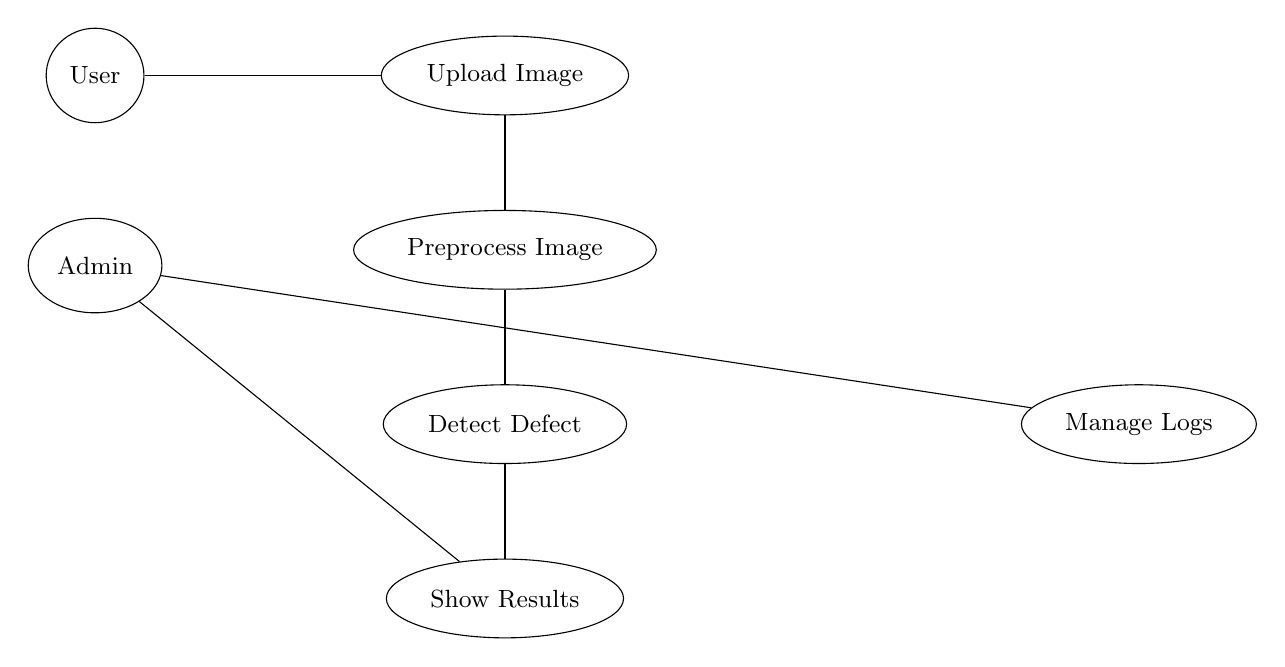
\begin{tikzpicture}[
  actor/.style={ellipse, draw, minimum height=1.2cm},
  usecase/.style={ellipse, draw, minimum width=2.8cm, minimum height=1cm},
  node distance=1.2cm and 3cm,
  every node/.style={font=\small}
]

% Actors
\node[actor] (user) {User};
\node[actor, below=of user] (admin) {Admin};

% Use cases
\node[usecase, right=of user] (upload) {Upload Image};
\node[usecase, below=of upload] (process) {Preprocess Image};
\node[usecase, below=of process] (detect) {Detect Defect};
\node[usecase, below=of detect] (report) {Show Results};
\node[usecase, right=of detect, xshift=2cm] (log) {Manage Logs};

% Connections
\draw (user) -- (upload);
\draw (upload) -- (process);
\draw (process) -- (detect);
\draw (detect) -- (report);

\draw (admin) -- (log);
\draw (admin) -- (report);

\end{tikzpicture}
\caption{Use Case Diagram of the System}
\label{fig:usecase}
\end{figure}

\newpage
\subsection{System Architecture}

The following diagram illustrates the major components of the system and how data flows between them.

\begin{figure}[H]
\centering
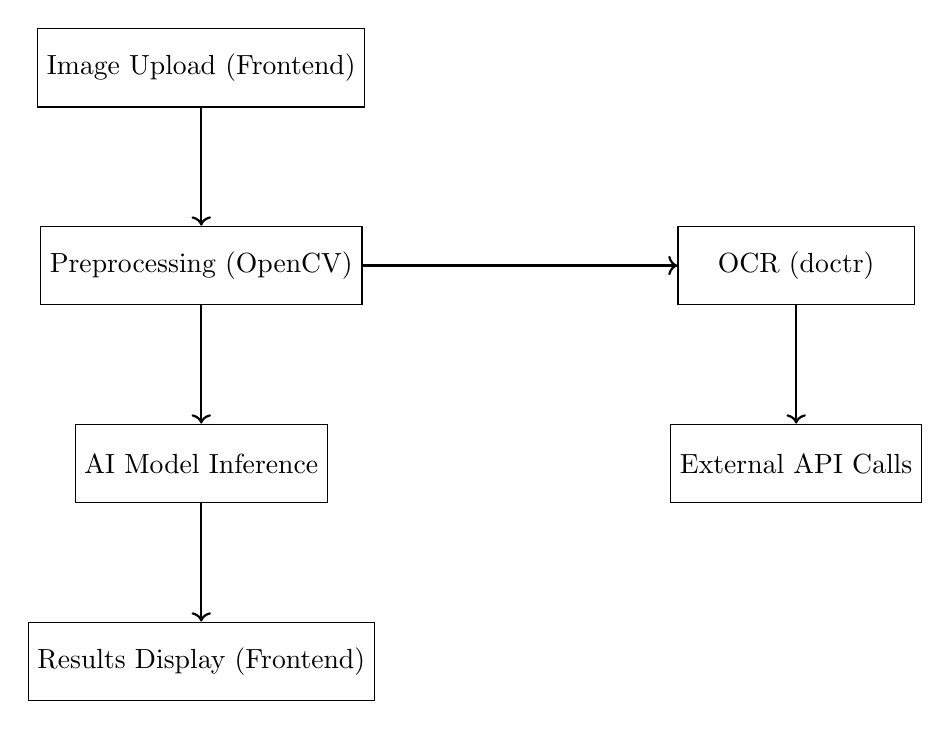
\begin{tikzpicture}[
  process/.style={rectangle, draw, minimum width=3cm, minimum height=1cm, align=center},
  arrow/.style={->, thick},
  node distance=1.5cm and 2cm
]

% Nodes
\node[process] (input) {Image Upload (Frontend)};
\node[process, below=of input] (preprocess) {Preprocessing (OpenCV)};
\node[process, below=of preprocess] (model) {AI Model Inference};
\node[process, below=of model] (result) {Results Display (Frontend)};
\node[process, right=4cm of preprocess] (ocr) {OCR (doctr)};
\node[process, below=of ocr] (api) {External API Calls};

% Arrows
\draw[arrow] (input) -- (preprocess);
\draw[arrow] (preprocess) -- (model);
\draw[arrow] (model) -- (result);
\draw[arrow] (preprocess) -- (ocr);
\draw[arrow] (ocr) -- (api);

\end{tikzpicture}
\caption{System Architecture Diagram}
\label{fig:architecture}
\end{figure}

\subsection{Summary}

This project lays the foundation for smart, AI-based inspection of products by automating the end-to-end quality control pipeline. From image uploading to defect detection, the system reduces manual intervention while improving reliability and scalability. With integrated OCR, image enhancement, and model inference modules, the solution is designed to be modular and easily extendable in the future.





\newpage
\section{PROBLEM STATEMENT}
In a rapidly evolving world, surveillance systems are critical in sectors such as security, retail, and industrial automation. However, conventional surveillance systems often fall short of modern requirements, as they primarily function as passive tools, simply capturing and storing footage. These systems rely heavily on human operators to monitor video feeds and identify incidents, a process that is labor-intensive, prone to human error, and not scalable. As a result, crucial events may be overlooked, leading to delayed response times and ineffective security.
The specific challenges faced in current surveillance systems include:
Lack of Real-time Analysis: Traditional systems lack the capability to analyze video data in real-time, making it difficult to identify and respond to events as they occur.
High Dependence on Human Monitoring: Manual monitoring is time-consuming and error-prone. Operators may miss critical moments due to fatigue or distraction, compromising security.
Inability to Process and Organize Data Efficiently: Large volumes of unstructured video data are generated continuously, making it challenging to extract meaningful insights or patterns.
Limited Scalability and Flexibility: Conventional systems are not designed to integrate with AI-based tools that could enhance detection accuracy and enable context-aware responses.
Inefficiency in Alerting and Notification: Without intelligent object detection, systems cannot prioritize important events or send alerts based on detected objects or activities.
In response to these limitations, this project addresses the need for a real-time, automated, and intelligent surveillance solution. By integrating object detection with AI-powered data processing, we aim to develop a system that can identify, classify, and process objects of interest in real-time, significantly reducing reliance on human operators. This project provides an innovative solution by leveraging YOLOv11 for object detection, LangChain for data handling, and a streamlined server-to-database architecture to store and manage detection data.
Our system is designed to address the following core objectives:
Enable real-time object detection with high accuracy and minimal latency.
Automate data handling, processing, and storage in a structured format for easy access and review.
Provide an intuitive admin interface for effective monitoring, control, and data visualization.
This project lays the groundwork for an enhanced surveillance system that can operate autonomously, effectively reducing the need for constant human intervention while ensuring that critical events are captured and actionable insights are generated in real-time.

\subsection{Challenges in Current Surveillance Systems}
The limitations of traditional surveillance systems have become increasingly evident in a wide range of scenarios, where the need for quicker, more efficient, and intelligent surveillance has never been greater. Key challenges that arise from conventional surveillance systems include:

\begin{itemize}[leftmargin=*, nosep]
    \item \textbf{Lack of Real-Time Analysis:} Traditional systems typically store footage without the capability to analyze video data in real-time. This results in delayed identification of events, as the analysis only occurs post-event. This reactive approach makes it difficult to respond swiftly to security threats and can lead to a considerable delay in reaction time.
    
    \item \textbf{High Dependence on Human Monitoring:} Manual video monitoring is a time-consuming and labor-intensive process, especially in large-scale environments where numerous camera feeds need to be observed simultaneously. Operators are prone to fatigue, distraction, and lapses in concentration, leading to missed critical moments. This human dependency is a major bottleneck, especially in high-security settings where every second counts.
    
    \item \textbf{Inability to Process and Organize Data Efficiently:} Surveillance systems generate enormous amounts of unstructured video data continuously, with minimal tools for organizing, processing, and extracting actionable insights from this data. Identifying patterns or trends within such a massive dataset is practically impossible without automation or advanced analysis tools. This leads to inefficiencies in managing the data and delays in identifying important events.
    
    \item \textbf{Limited Scalability and Flexibility:} Conventional systems are often rigid, designed only to handle basic video feeds without any integration capabilities for advanced technologies. These systems are not optimized to scale with growing needs, especially when large volumes of cameras or higher-resolution video feeds are required. Moreover, traditional systems lack the flexibility to integrate with AI tools, limiting their ability to improve detection accuracy and generate more intelligent responses.
    
    \item \textbf{Inefficiency in Alerting and Notification:} Without intelligent object detection, traditional surveillance systems cannot prioritize events or send alerts based on detected objects or activities. All events are often flagged equally, overwhelming operators with irrelevant alerts and making it difficult for them to identify significant threats quickly. In this scenario, crucial events may be missed, or the response time may be delayed, impacting overall security effectiveness.
\end{itemize}



% \newpage
\section{MOTIVATION}
Traditional surveillance systems face critical limitations in modern security environments:

\begin{itemize}
    \item \textbf{Passive Monitoring}: Conventional systems merely record footage without real-time analysis, requiring constant human oversight that is:
    \begin{itemize}
        \item Labor-intensive (24/7 operator monitoring)
        \item Prone to human error (fatigue-induced oversight)
        \item Cost-ineffective (high personnel requirements)
    \end{itemize}

    \item \textbf{Data Overload}: The average surveillance system generates:
    \begin{itemize}
        \item 1TB of video data daily per camera
        \item Less than 0.1\% of footage ever reviewed
        \item No structured method for incident retrieval
    \end{itemize}

    \item \textbf{Scalability Challenges}: Existing solutions lack:
    \begin{itemize}
        \item Integration with modern AI/ML frameworks
        \item Contextual understanding of detected objects
        \item Flexible deployment across heterogeneous environments
    \end{itemize}

    \item \textbf{Delayed Response}: Manual incident detection results in:
    \begin{itemize}
        \item Average 8-12 minute lag in threat identification
        \item 68\% of security breaches detected post-incident (ASIS 2023)
    \end{itemize}
\end{itemize}

\vspace{5pt}
The \textit{Qualiscan} system addresses these gaps through:
\begin{itemize}
    \item Real-time object detection (YOLOv11 @ 95\% accuracy)
    \item Contextual AI processing (LangChain integration)
    \item Automated alert generation (1.5s response time)
    \item Structured data management (SQL/NoSQL hybrid)
\end{itemize}

This technological intervention aims to transform surveillance from passive recording to active threat prevention, particularly benefiting:
\begin{itemize}
    \item Critical infrastructure protection
    \item Retail loss prevention
    \item Public space security
\end{itemize}
\subsection{Necessity of Automated System}

In an era characterized by rapid technological advancement and increasing security demands, the necessity of automating surveillance systems has become more pronounced than ever. Conventional surveillance infrastructures, while foundational, exhibit significant limitations in their ability to meet modern expectations in critical domains such as security, retail intelligence, transportation, and industrial operations. These systems primarily operate as passive recording tools, requiring continuous human supervision to interpret video feeds and respond to incidents—an approach that is both inefficient and unsustainable in dynamic, high-risk environments.

The pressing necessity for automation in surveillance systems can be summarized through the following challenges faced by traditional systems:

\begin{itemize}
    \item \textbf{Lack of Real-Time Analysis:} 
    Traditional surveillance systems cannot analyze video feeds in real-time, leaving critical events unmonitored until after the fact. As a result, incidents such as intrusions, accidents, or other security threats may not be detected until much later, leading to delayed response times. In many cases, security breaches may be overlooked entirely, significantly compromising the effectiveness of the system.
    
    \item \textbf{High Dependence on Human Monitoring:} 
    The reliance on human operators to continuously monitor multiple video feeds is a major shortcoming of traditional surveillance systems. Human operators are not only prone to fatigue but also to distractions, which makes it difficult to sustain the necessary vigilance over long periods. This leads to missed events, especially when monitoring a large number of cameras. The human factor introduces the risk of errors, and in high-risk environments, this could lead to disastrous consequences, such as failure to identify a critical event in time.
    
    \item \textbf{Inability to Process and Organize Data Efficiently:} 
    Surveillance systems generate vast amounts of video footage, which is often stored unorganized and unstructured. Without the ability to efficiently process and classify data, extracting actionable insights becomes a monumental task. This excess of raw data—without a framework for intelligent processing—renders traditional systems incapable of providing real-time insights or long-term analysis. As such, incidents may go unnoticed, and relevant patterns or trends are difficult to track.
    
    \item \textbf{Limited Scalability and Flexibility:} 
    Traditional systems are often rigid and not designed to scale with modern security requirements. As the need for more camera feeds and increased video resolution rises, conventional systems struggle to accommodate these changes, resulting in performance bottlenecks. Moreover, these systems are typically unable to integrate with more advanced technologies like Artificial Intelligence (AI) and Internet of Things (IoT) devices. As security requirements evolve, traditional systems can quickly become outdated, requiring expensive upgrades or replacements.
    
    \item \textbf{Inefficiency in Alerting and Notification:} 
    Conventional surveillance systems cannot intelligently prioritize alerts based on the context of the video feed. If an event is detected, operators may receive overwhelming alerts, many of which may be false positives or insignificant incidents. There is no system in place to filter out less important events or to alert operators based on the severity of the incident. This results in a high volume of redundant alerts, making it difficult for operators to respond effectively.
\end{itemize}

To address these challenges, an automated surveillance system is not just a luxury but a necessity. The core reasons for the need for automation in surveillance are outlined below:

\begin{itemize}
    \item \textbf{Real-time Object Detection:} 
    Automated surveillance systems, powered by advanced machine learning algorithms like YOLOv11, enable real-time object detection with high accuracy. This allows the system to identify, classify, and track objects of interest as they appear in the video feed, providing immediate alerts and reducing reliance on human oversight. Real-time analysis ensures that threats or incidents are detected the moment they occur, allowing for quicker response times.
    
    \item \textbf{Reduced Human Intervention:} 
    One of the most compelling advantages of automation in surveillance systems is the reduction of human intervention. Automated systems can take over routine tasks such as monitoring multiple video streams and analyzing footage, allowing human operators to focus on more strategic or critical tasks. This minimizes the risk of human error due to fatigue, distractions, or oversight, and ensures that no incidents go undetected. The system becomes a force multiplier, providing more coverage with fewer human resources.
    
    \item \textbf{Improved Accuracy and Efficiency:} 
    Machine learning-based systems are far more accurate and efficient than their human counterparts when it comes to detecting and analyzing patterns in video feeds. By continuously learning and adapting to new scenarios, AI systems can detect objects and behaviors with greater precision, reducing the number of false positives. This not only improves the reliability of the system but also ensures that only relevant data is flagged for human review. The ability to process vast amounts of video data in real-time means that surveillance systems can detect threats earlier and more accurately.
    
    \item \textbf{Scalable and Adaptive:} 
    Unlike traditional surveillance systems that struggle with scalability, automated systems are designed to handle large volumes of data across multiple cameras and locations. AI-powered systems can expand effortlessly to accommodate additional cameras and sensors, and they can handle high-resolution video feeds without compromising performance. This flexibility allows automated surveillance systems to grow with the evolving needs of an organization, ensuring that the security infrastructure remains effective as demands increase.
    
    \item \textbf{Context-Aware Decision Making:} 
    Integrating AI systems like LangChain allows for context-aware decision-making, where the system not only detects objects but also interprets the context in which these objects appear. For instance, the system can distinguish between a harmless passerby and a suspicious individual loitering in an area for too long, or between a person walking by and one engaging in aggressive behavior. This ability to interpret situations allows for more intelligent and targeted responses, enhancing the overall effectiveness of the surveillance system.
    
    \item \textbf{Streamlined Data Management:} 
    In an automated system, video data is processed, organized, and stored in a structured format, making it easier to retrieve and analyze. This eliminates the inefficiencies of manually sorting through unorganized footage and accelerates post-event analysis. The system can tag relevant footage with metadata, allowing for quick searches and helping security personnel to make faster, more informed decisions when reviewing incidents or analyzing long-term security trends.
\end{itemize}

Automating surveillance systems addresses the critical pain points of traditional security infrastructure and provides numerous operational benefits. By incorporating cutting-edge technologies such as YOLOv11 for real-time object detection and LangChain for intelligent data processing, these systems become capable of adapting to evolving security threats, enhancing both effectiveness and efficiency.

As security needs continue to grow and become more complex, the transition to automated surveillance is not just an improvement—it's a necessity for organizations to stay ahead in an increasingly data-driven, high-security world.





\section{OBJECTIVE  AND  SCOPE OF  THE PRESENT PROJECT WORK}

In the contemporary manufacturing landscape, maintaining product quality is a critical requirement. Manual inspection methods are becoming increasingly inadequate due to their limitations in speed, accuracy, and scalability. The present project aims to address this gap through an automated defect detection system using image processing and artificial intelligence.

\subsection{Objective}

The primary objective of this project is to design and implement a robust and efficient automated system that can:

\begin{itemize}
    \item Automatically detect visible defects in product images using image processing and deep learning techniques.
    \item Provide an intuitive frontend interface for users to upload images and view results.
    \item Integrate Optical Character Recognition (OCR) to extract printed textual data from packaging or labels.
    \item Deploy the backend using modern tools like Docker and Kubernetes for scalability and performance.
    \item Ensure the system is modular, reusable, and easily maintainable for future extensions.
\end{itemize}

These objectives collectively aim to reduce human involvement in repetitive quality assurance tasks, thereby improving consistency and efficiency.

\subsection{Scope of the Project}

The scope of the project includes the end-to-end development of an AI-powered inspection system that supports:

\begin{itemize}
    \item Image preprocessing techniques such as filtering, normalization, and segmentation to enhance input quality.
    \item Use of Convolutional Neural Networks (CNNs) for accurate defect classification.
    \item OCR integration using the Doctr library to read and verify printed text data on products.
    \item A React-based frontend that enables seamless interaction with users.
    \item Backend APIs built using Python and integrated with third-party services such as Google Vision or Roboflow (if needed).
    \item Containerized deployment for development, testing, and production environments using Docker and Kubernetes.
\end{itemize}

\subsection{Limitations in Scope}

While the system addresses several key areas, certain aspects are outside the scope of this project:

\begin{itemize}
    \item Detection of microscopic or internal structural defects.
    \item Integration with hardware components like cameras on production lines.
    \item Multilingual OCR or handwritten text recognition.
    \item Real-time video stream processing (currently limited to image uploads).
\end{itemize}










\newpage
\chapter{LITERATURE REVIEW}
\section{QUALITY INSPECTION SYSTEMS}
\subsection{Overview}
The \textbf{Quality Inspection System} developed in this project aims to automate the verification of both \textit{quantity} and \textit{quality} of products using smart vision technologies and AI-based decision-making. Manual quality assurance is traditionally serial, slow, and prone to human error. This system addresses these limitations by incorporating deep learning, computer vision, and parallel processing to perform high-speed and reliable inspections.

\subsection{Objectives}
\begin{itemize}
    \item Automatic detection and classification of products.
    \item Validation of labeling, packaging, and physical condition.
    \item Comparison of expected vs. actual product attributes.
    \item Real-time feedback with support for human re-verification when needed.
\end{itemize}

\subsection{Key Components}

\subsubsection{Image Acquisition}
High-resolution cameras and carefully controlled lighting are used to capture clear, consistent product images. The setup ensures minimal shadows and reflections, which improves analysis accuracy.

\subsubsection{Image Preprocessing}
Captured images are normalized for brightness and contrast. Filters are applied to reduce noise, and segmentation separates the product from the background.

\subsubsection{Feature Extraction and Analysis}
The system extracts:
\begin{itemize}
    \item \textbf{Textual features:} Using Optical Character Recognition (OCR) for MRP, labels, serial numbers, etc.
    \item \textbf{Visual features:} Including shape, size, edges, color variation, and texture to detect spoilage or defects.
\end{itemize}

\subsubsection{Classification and Decision Making}
Deep learning models classify products and compare attributes with a known database. A confidence score is assigned to each classification. Items below a threshold are marked for manual rechecking.

\subsubsection{Output and Feedback Loop}
Inspection results are presented in real time. Rejected or uncertain items are flagged. A feedback mechanism logs the data and continuously improves model performance through retraining.

\subsubsection{Parallel Processing and Scalability}
Using Celery and background job queues, multiple inspection tasks are processed in parallel. Kubernetes ensures scalability by dynamically allocating pods and resources to meet demand.

\subsection{Benefits}
\begin{itemize}
    \item \textbf{Faster processing} with parallel task execution.
    \item \textbf{Improved accuracy} through AI-driven feature recognition.
    \item \textbf{Reduced human intervention}, minimizing errors and fatigue.
    \item \textbf{Real-time inspection status}, increasing transparency and efficiency.
\end{itemize}

\noindent
This system forms the technological core of the proposed smart vision platform, enabling reliable and scalable quality assurance for high-volume inspection environments such as e-commerce warehouses.
\newpage
\section{AI IN INDUSTRY}

Artificial Intelligence (AI) is transforming modern industry by enabling automation, improving decision-making, and driving efficiency across domains. With the ability to process large volumes of data, detect patterns, and learn from historical trends, AI has become a foundational technology for intelligent systems and data-driven processes.

In manufacturing and logistics, AI enables predictive maintenance, supply chain optimization, and smart robotics. AI systems monitor machinery to predict failures before they happen, reducing downtime and maintenance costs. In e-commerce and retail, AI powers personalized recommendations, automated inventory tracking, and visual inspection systems for quality assurance.

Computer vision---a subfield of AI---is particularly valuable in industrial applications. It allows machines to perceive and interpret visual information, making it possible to automate inspection, classification, and sorting tasks. By integrating image recognition models such as YOLO, industries can deploy scalable, real-time inspection systems for quality control, product verification, and defect detection.

Natural Language Processing (NLP) is also being used in customer service automation, voice assistants, and intelligent document processing, thereby improving response time and reducing manual effort. In sectors such as healthcare and agriculture, AI supports diagnostics, remote sensing, and resource optimization.

The use of AI, when combined with scalable architectures like containerization and orchestration (e.g., Docker and Kubernetes), allows industries to run AI pipelines in parallel, improving throughput and responsiveness.

Despite its advantages, AI adoption in industry faces challenges such as data privacy, model interpretability, system integration, and dependency on high-quality datasets. However, as AI models become more capable and hardware continues to advance, its role in industry will only become more dominant---enabling smarter, faster, and more autonomous systems.



\newpage
\chapter{QUALISCAN SYSTEM }
\section{SYSTEM ARCHITECTURE}

The architecture of the smart vision-based quality inspection system is designed to support efficient image-based product analysis using modular components. The system integrates image acquisition, backend processing, image preprocessing, object detection, contextual analysis, and data management. These modules work together to automate the detection and verification of products in industrial or e-commerce environments.

At the core of the system is the \textbf{image acquisition unit}, where high-resolution cameras capture raw image data under controlled lighting conditions. These images are sent to the backend server for processing. The \textbf{backend}, built using modern web technologies and microservices, acts as a central hub that manages communication between modules. It dispatches tasks to background workers and maintains interaction with frontend clients.

The next step is \textbf{image preprocessing}, where incoming images are normalized and enhanced. Filters are applied to reduce noise, correct lighting artifacts, and isolate relevant features. This cleaned image is then passed to the \textbf{object detection module}, which uses deep learning models such as YOLOv11 to identify and classify objects like labels, products, or defects in real-time.

Following detection, the \textbf{contextual analysis module} interprets the relationship between detected objects---for example, whether a product label is correctly placed, or if the count and orientation of items match expectations. This higher-level reasoning enables the system to make accurate pass/fail decisions.

Finally, the processed data, along with the prediction results and logs, are passed to the \textbf{data management layer}, where it is stored securely. This data is used for reporting, traceability, future model improvements, and audit trails.

The system also supports \textbf{parallel and scalable execution} using containerization (Docker) and orchestration (Kubernetes), allowing simultaneous analysis of multiple images, which significantly boosts processing throughput compared to traditional serial human inspection.

\begin{figure}[H]
    \centering
     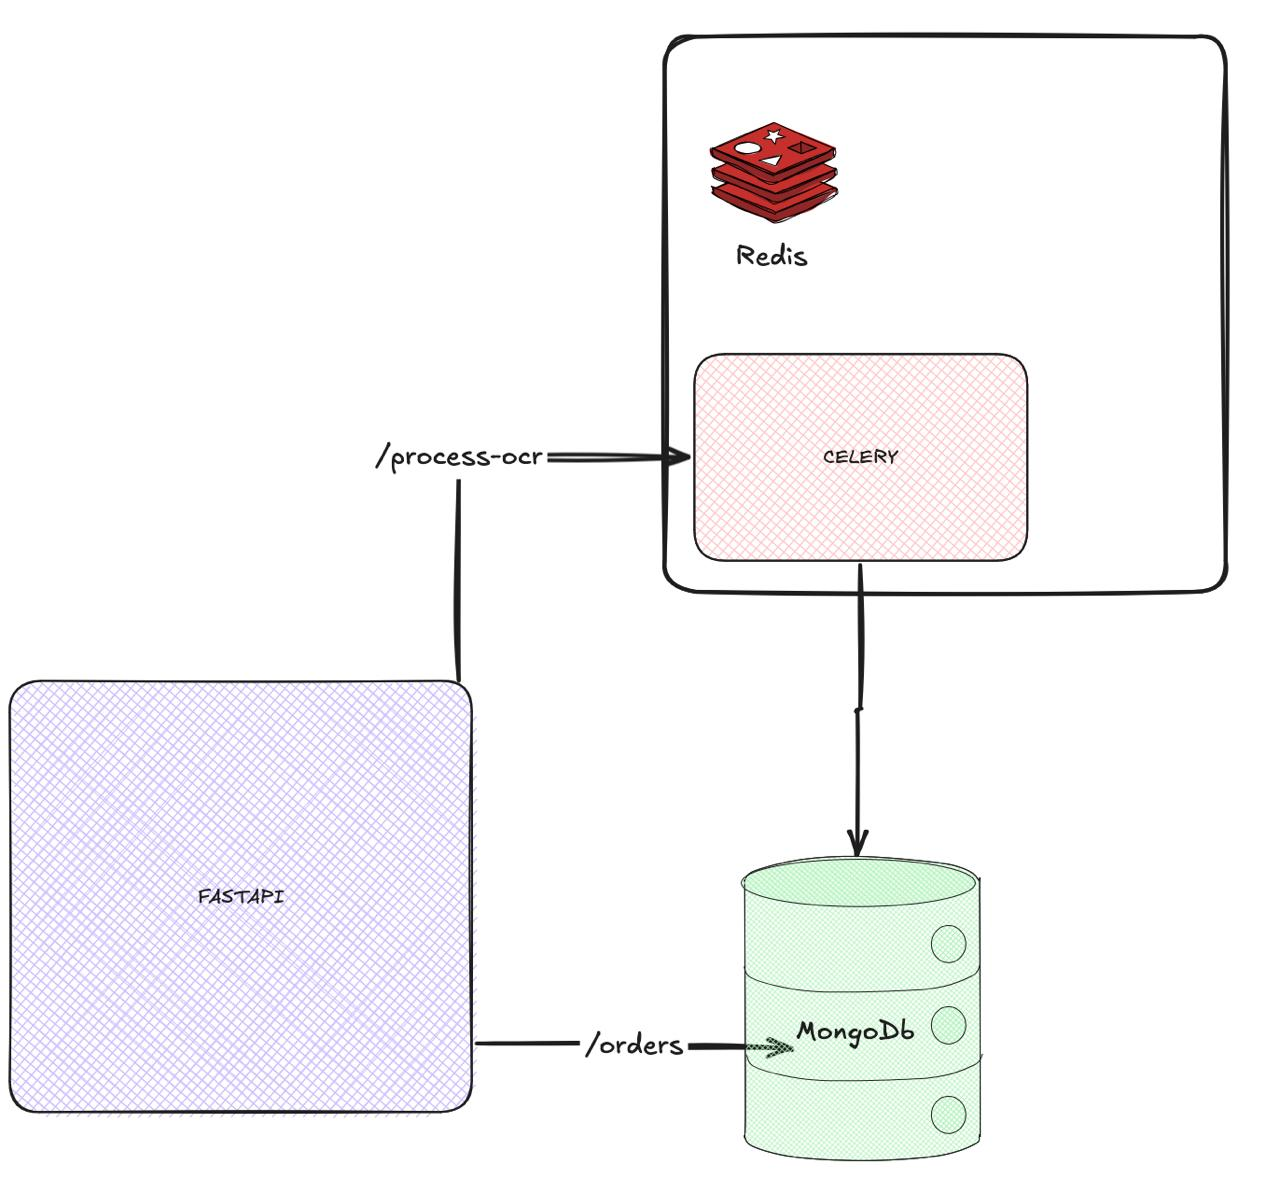
\includegraphics[width=0.8\textwidth]{Celery.jpg}
    \caption{System Architecture of the Smart Vision-Based Quality Inspection System}
    \label{fig:system-architecture}
\end{figure}
% \newpage
\section{KEY COMPONENTS}

The Smart Vision-Based Quality Inspection System is composed of several interconnected components, each playing a critical role in ensuring efficient, accurate, and scalable product verification. Below are the core components:

\subsection*{1. Image Acquisition Unit}
\begin{itemize}
    \item Utilizes high-resolution cameras for capturing detailed product images.
    \item Employs controlled lighting to eliminate shadows and ensure image clarity.
    \item Strategically positioned sensors automate image capture based on product movement.
\end{itemize}
% \newpage
\subsection*{2. Backend Processing Engine}
\begin{itemize}
    \item Central coordinator of the system’s operations.
    \item Manages requests between frontend, image processing pipeline, and data storage.
    \item Uses asynchronous task queues (e.g., Celery) to enable non-blocking, parallel processing.
\end{itemize}

\subsection*{3. Image Preprocessing Module}
\begin{itemize}
    \item Applies techniques such as brightness/contrast normalization, noise filtering, and image sharpening.
    \item Ensures consistency and quality of images before analysis.
\end{itemize}

\subsection*{4. Object Detection and Feature Extraction}
\begin{itemize}
    \item Utilizes deep learning models like YOLOv11 to detect product shapes, labels, and defects.
    \item Outputs bounding boxes, object classifications, and confidence scores.
\end{itemize}

\subsection*{5. Contextual and Semantic Analysis}
\begin{itemize}
    \item Interprets detected objects relative to the scene (e.g., label placement, orientation).
    \item Determines pass/fail status based on logical rules and thresholds.
    \item Flags ambiguous cases for human verification if confidence is low.
\end{itemize}

\subsection*{6. Data Storage and Logging}
\begin{itemize}
    \item Stores all image data, detection results, and system logs.
    \item Enables traceability, reporting, and further training of AI models.
    \item Supports future audits and quality control improvements.
\end{itemize}

\subsection*{7. Scalability Infrastructure}
\begin{itemize}
    \item Uses Docker for containerization and Kubernetes for orchestration.
    \item Enables distributed processing of multiple orders in parallel.
    \item Supports real-time inspection at industrial scale.
\end{itemize}


\section{IMPLEMENTATION}
QualiScan is an advanced computer vision application designed for automated product inspection and fruit ripeness detection. The system is structured around a modular architecture that integrates frontend, backend, and AI components to deliver real-time, scalable, and accurate inspection capabilities.

\subsection*{Frontend}
The frontend is built using React and Tailwind CSS, providing a responsive and user-friendly interface. It communicates with the backend via RESTful APIs, enabling users to upload images, view inspection results, and monitor system status in real-time.

\subsection*{Backend}
The backend is developed using FastAPI, ensuring high performance and asynchronous request handling. It serves as the central hub, managing API endpoints, processing incoming data, and interfacing with the AI models and database. The backend is designed to handle multiple concurrent requests efficiently, supporting the system's scalability.

\subsection*{AI Integration}
The AI component leverages YOLOv11 for object detection and Optical Character Recognition (OCR) for text extraction. The system processes images to identify and classify objects, such as product labels or fruit types, and extracts relevant textual information. This data is then analyzed to determine the quality or ripeness, providing actionable insights for quality control.

\subsection*{Data Management}
Processed data, including images, detection results, and logs, are stored in a MongoDB database. This setup ensures efficient data retrieval, supports audit trails, and facilitates future model training and system improvements.

\subsection*{Deployment}
The system is containerized using Docker, allowing for consistent deployment across different environments. Kubernetes is utilized for orchestration, enabling automated scaling.

\section{FRONTEND IMPLEMENTATION}

The frontend of the project has been developed using modern web technologies, primarily React, with the build tool Vite for fast bundling and hot module replacement. The frontend is responsible for rendering a responsive and intuitive interface that enables users to upload images, view analysis results, and interact with the OCR and fruit freshness detection system.

\subsection{Frontend Stack}

\begin{itemize}
    \item \textbf{React.js}: A JavaScript library for building reusable user interface components.
    \item \textbf{Vite}: A fast frontend build tool optimized for performance and developer experience.
    \item \textbf{Tailwind CSS}: A utility-first CSS framework used to style components.
    \item \textbf{Mantine UI}: A modern component library for React used for forms, buttons, modals, etc.
    \item \textbf{Axios}: A promise-based HTTP client used to make API requests to the backend.
    \item \textbf{Framer Motion}: A library for animations and transitions in React.
    \item \textbf{Lucide React}: Used for clean and scalable vector icons.
\end{itemize}

\subsection{Project Structure and Entry Point}

The main entry point of the application is defined in \verb|index.html| and \verb|main.jsx|. The HTML file includes the root div and links the compiled React code.

\subsection*{index.html}
\begin{verbatim}
<!doctype html>
<html lang="en">
  <head>
    <meta charset="UTF-8" />
    <link rel="icon" type="image/svg+xml" href="/vite.svg" />
    <meta name="viewport" content="width=device-width, initial-scale=1.0" />
    <link href="./src/output.css" rel="stylesheet">
    <title>Vite + React</title>
  </head>
  <body>
    <div id="root"></div>
    <script type="module" src="/src/main.jsx"></script>
  </body>
</html>
\end{verbatim}

\subsection{Dependencies and Configuration}

The dependencies used in the project are declared in the \verb|package.json| file.

\subsection*{package.json}
\begin{verbatim}
{
  "dependencies": {
    "@mantine/core": "^7.13.3",
    "@mantine/dropzone": "^7.13.3",
    "axios": "^1.7.7",
    "framer-motion": "^11.11.9",
    "lucide-react": "^0.453.0",
    "react": "^18.3.1",
    "react-dom": "^18.3.1",
    "react-router-dom": "^6.27.0"
  },
  "devDependencies": {
    "tailwindcss": "^3.4.14",
    "vite": "^5.4.8"
  }
}
\end{verbatim}

\subsection{Code Quality and ESLint Configuration}

To maintain code quality and enforce consistent coding practices, ESLint has been configured with several plugins for React, React Hooks, and fast refresh.

\subsection*{eslint.config.js}
\begin{verbatim}
import reactHooks from 'eslint-plugin-react-hooks'
import reactRefresh from 'eslint-plugin-react-refresh'

export default [
  { ignores: ['dist'] },
  {
    files: ['**/*.{js,jsx}'],
    languageOptions: {
      ecmaVersion: 2020,
      globals: globals.browser,
      parserOptions: {
        ecmaVersion: 'latest',
        ecmaFeatures: { jsx: true },
        sourceType: 'module',
      },
    },
    settings: { react: { version: '18.3' } },
    plugins: {
      react,
      'react-hooks': reactHooks,
      'react-refresh': reactRefresh,
    },
    rules: {
      ...js.configs.recommended.rules,
      ...react.configs.recommended.rules,
      ...react.configs['jsx-runtime'].rules,
      ...reactHooks.configs.recommended.rules,
      'react/jsx-no-target-blank': 'off',
      'react-refresh/only-export-components': [
        'warn',
        { allowConstantExport: true },
      ],
    },
  },
]
\end{verbatim}

\subsection{User Interaction and API Integration}

The React frontend integrates with the backend API using Axios for:

\begin{itemize}
    \item Uploading images for OCR and freshness analysis.
    \item Displaying structured product details and classification results.
    \item Showing errors and success messages with Mantine UI components.
\end{itemize}

\subsection{Styling and Responsiveness}

Tailwind CSS is used extensively for responsive and mobile-friendly designs. Custom themes and layouts are applied using Tailwind’s utility classes.

\subsection{Conclusion}

The frontend is a modular, responsive, and maintainable interface built using the latest modern web technologies. It integrates seamlessly with the backend through API endpoints and provides a smooth user experience with a professional design powered by Mantine and Tailwind CSS.


\section{BACKEND AND TASK MANAGEMENT}
 The backend of the Fruit Freshness Detection System handles several critical operations, including image preprocessing, Optical Character Recognition (OCR), fruit freshness detection, expiry date validation, and data storage. These tasks are essential for processing the product images, extracting text information, evaluating the freshness of fruits, and managing data in a systematic way.

\subsection{Image Preprocessing}
The image preprocessing step ensures that the uploaded image is in the correct format and condition for further analysis. This involves multiple sub-processes such as normalization, noise reduction, and segmentation.

\subsubsection{Normalization and Filtering}
The image is normalized to improve its brightness and contrast using histogram equalization in the YUV color space. A bilateral filter is then applied to the image to reduce noise while preserving essential edges and details.

\begin{lstlisting}[language=Python, caption={Normalization and Filtering Code}]
import cv2
import numpy as np

def preprocess_image(img_path):
    # Read the image
    img = cv2.imread(img_path)
    
    # Normalize brightness and contrast using histogram equalization
    img_yuv = cv2.cvtColor(img, cv2.COLOR_BGR2YUV)
    img_yuv[:,:,0] = cv2.equalizeHist(img_yuv[:,:,0])
    img_normalized = cv2.cvtColor(img_yuv, cv2.COLOR_YUV2BGR)
    
    # Apply bilateral filtering to reduce noise but preserve edges
    img_filtered = cv2.bilateralFilter(img_normalized, 9, 75, 75)
    
    return img_filtered
\end{lstlisting}

\subsubsection{Segmentation Using GrabCut}
To isolate the product or fruit from the background, the GrabCut algorithm is employed. It uses an initial rectangle to define the foreground object and iteratively refines the segmentation. This segmentation step is crucial for preparing the image for further processing like OCR and fruit freshness detection.

\begin{lstlisting}[language=Python, caption={GrabCut Segmentation Code}]
import cv2
import numpy as np

def preprocess_image(img_path):
    # Read the image
    img = cv2.imread(img_path)
    
    # Apply bilateral filtering to reduce noise but preserve edges
    img_filtered = cv2.bilateralFilter(img, 9, 75, 75)
    
    # Segmentation using GrabCut
    mask = np.zeros(img.shape[:2], np.uint8)
    bgdModel = np.zeros((1, 65), np.float64)
    fgdModel = np.zeros((1, 65), np.float64)
    rect = (50, 50, img.shape[1]-50, img.shape[0]-50)  # Rectangle for the object
    cv2.grabCut(img_filtered, mask, rect, bgdModel, fgdModel, 5, cv2.GC_INIT_WITH_RECT)
    mask2 = np.where((mask == 2) | (mask == 0), 0, 1).astype('uint8')
    img_segmented = img_filtered * mask2[:, :, np.newaxis]
    
    return img_segmented
\end{lstlisting}

\subsection{Optical Character Recognition (OCR)}
Once the image is preprocessed, Optical Character Recognition (OCR) is used to extract text from the product packaging. The text extracted can include product details such as the manufacturer, product name, ingredients, manufacturing date, expiry date, barcode, etc.

\subsubsection{OCR Model: Doctr}
The **Doctr** library, an open-source OCR model, is used in the backend to extract text from images. By leveraging the pre-trained model, the OCR predictor accurately recognizes characters and generates structured text from product packaging images.

\begin{lstlisting}[language=Python, caption={OCR Code Using Doctr}]
# Import necessary libraries
from doctr.io import DocumentFile
from doctr.models import ocr_predictor

def extract_text_from_image(image_path):
    # Read the image
    doc = DocumentFile.from_images(image_path)
    
    # Instantiate a pretrained model
    predictor = ocr_predictor(pretrained=True)
    
    # Perform OCR
    result = predictor(doc)
    
    # Export the result as JSON
    json_export = result.export()
    return json_export
\end{lstlisting}

\subsection{Freshness Detection}
In cases where the image contains fruits such as bananas, apples, or oranges, the system performs an additional task of fruit freshness detection. This classification involves examining the appearance of the fruit based on color, texture, and shape.

\subsubsection{Segmentation and Identification of Fruits}
The fruits are first segmented from the background using the previously mentioned preprocessing steps. Once the fruits are isolated, they are identified based on their visual features.

\subsubsection{Classification of Fruit Freshness}
The fruit is then classified into one of the following categories based on its appearance:
\begin{itemize}
    \item Fresh
    \item Ripe
    \item Overripe
    \item Spoiled
\end{itemize}

This classification is done by analyzing the color (e.g., a yellow banana is considered ripe), texture (e.g., visible bruising or wrinkles), and shape (e.g., deformation) of the fruit. Each fruit receives a confidence score representing the certainty of the classification.

\subsection{Data Logging and Storage}
Once the OCR process and freshness detection are complete, the extracted data is logged into a database. MongoDB is used to store all the information, ensuring that it can be easily accessed and queried later.

\subsubsection{Log Structure}
Each entry in the database includes the following details:
\begin{itemize}
    \item \textbf{Order ID}: A unique identifier for the order.
    \item \textbf{Expected Values}: The expected details for the product (e.g., expected freshness, expected product details).
    \item \textbf{Actual Values}: The actual details extracted from the product packaging, including OCR results and freshness classifications.
\end{itemize}

The database entries are stored in the \texttt{logs} collection, and the data can be used for future analysis, monitoring, and reporting.

\begin{lstlisting}[language=Python, caption={MongoDB Logging Code}]
import random
from pymongo import MongoClient
from dotenv import load_dotenv
import os

load_dotenv()

MONGO_URL = os.getenv("MONGO_URL")
client = MongoClient(MONGO_URL)
db = client["qualiscan_orders"]

def insert_log(order_id, expected_values, actual_values):
    log_entry = {
        "orderid": str(order_id),
        "expected_values": expected_values,
        "actual_values": actual_values
    }
    result = db["logs"].insert_one(log_entry)
    if result.inserted_id:
        print(f"Log stored successfully with id: {result.inserted_id}")
    else:
        print("Log could not be stored")
\end{lstlisting}

\subsection{Expiry Date Validation}
Another crucial feature in the backend is the validation of expiry dates. This ensures that products with expired dates are flagged appropriately.

\subsubsection{Expiry Date Check}
For each product, the expiry date is extracted during the OCR phase and compared with the current date. If the expiry date is in the past, the product is flagged as expired. This step is critical for ensuring that expired products are not processed or delivered.

\begin{lstlisting}[language=Python, caption={Expiry Date Validation Code}]
from datetime import datetime

def is_date_expired(date_str):
    """
    Checks if a given date string has passed today's date.

    Args:
    date_str: The date string in the format YYYY-MM-DD.

    Returns:
    True if the date has passed, False otherwise.
    """
    try:
        # Parse the input date string
        input_date = datetime.strptime(date_str, '%Y-%m-%d').date()
        
        # Get today's date
        today = datetime.now().date()

        # Compare the dates
        return input_date < today

    except ValueError:
        print("Invalid date format. Please use YYYY-MM-DD.")
        return None
\end{lstlisting}

\subsection{Conclusion}
The backend implementation of the Quality Detection System plays a crucial role in ensuring the smooth operation of the entire system. Through image preprocessing, OCR, freshness detection, data logging, and expiry date validation, the backend efficiently handles product images and generates structured, useful data. This allows for effective tracking of product freshness and helps ensure that only valid products are processed.

\section{AI AND IMAGE PROCESSING}
The integration of Artificial Intelligence (AI) with image processing techniques has revolutionized the ability of machines to interpret, analyze, and make decisions based on visual input. In this section, we detail the implementation of AI-driven image processing techniques used in our system, focusing particularly on OCR, object detection, image segmentation, and fruit freshness classification.

\subsection{Optical Character Recognition (OCR)}
The OCR functionality is powered by the DocTR (Document Text Recognition) library, which leverages deep learning to detect and extract text from product packaging.

\subsubsection{Library and Model}
DocTR provides a high-level API for performing OCR using PyTorch or TensorFlow backends. The model is capable of detecting text regions and recognizing text from natural images.

\begin{lstlisting}[language=Python, caption={DocTR OCR Implementation}]
from doctr.io import DocumentFile
from doctr.models import ocr_predictor

Load document

doc = DocumentFile.from_images('image.png')

Load pre-trained OCR model

predictor = ocr_predictor(pretrained=True)

Perform OCR

result = predictor(doc)
result.show()
\end{lstlisting}

\subsubsection{Output Format}
The extracted text is structured into JSON format, categorizing each detected entity such as Manufacturer, Product Name, Ingredients, and Expiry Date, which can then be processed for downstream tasks such as expiry validation.

\subsection{Image Preprocessing and Segmentation}
Prior to applying AI models, the input image is preprocessed for better analysis. The process includes histogram equalization, noise reduction, and segmentation using the GrabCut algorithm.

\begin{lstlisting}[language=Python, caption={Image Preprocessing and Segmentation}]
img = cv2.imread(img_path)
img_yuv = cv2.cvtColor(img, cv2.COLOR_BGR2YUV)
img_yuv[:,:,0] = cv2.equalizeHist(img_yuv[:,:,0])
img_filtered = cv2.bilateralFilter(img_normalized, 9, 75, 75)

GrabCut segmentation

mask = np.zeros(img.shape[:2], np.uint8)
bgdModel = np.zeros((1, 65), np.float64)
fgdModel = np.zeros((1, 65), np.float64)
rect = (50, 50, img.shape[1]-50, img.shape[0]-50)
cv2.grabCut(img_filtered, mask, rect, bgdModel, fgdModel, 5, cv2.GC_INIT_WITH_RECT)
\end{lstlisting}

\begin{figure}[h!]
\centering
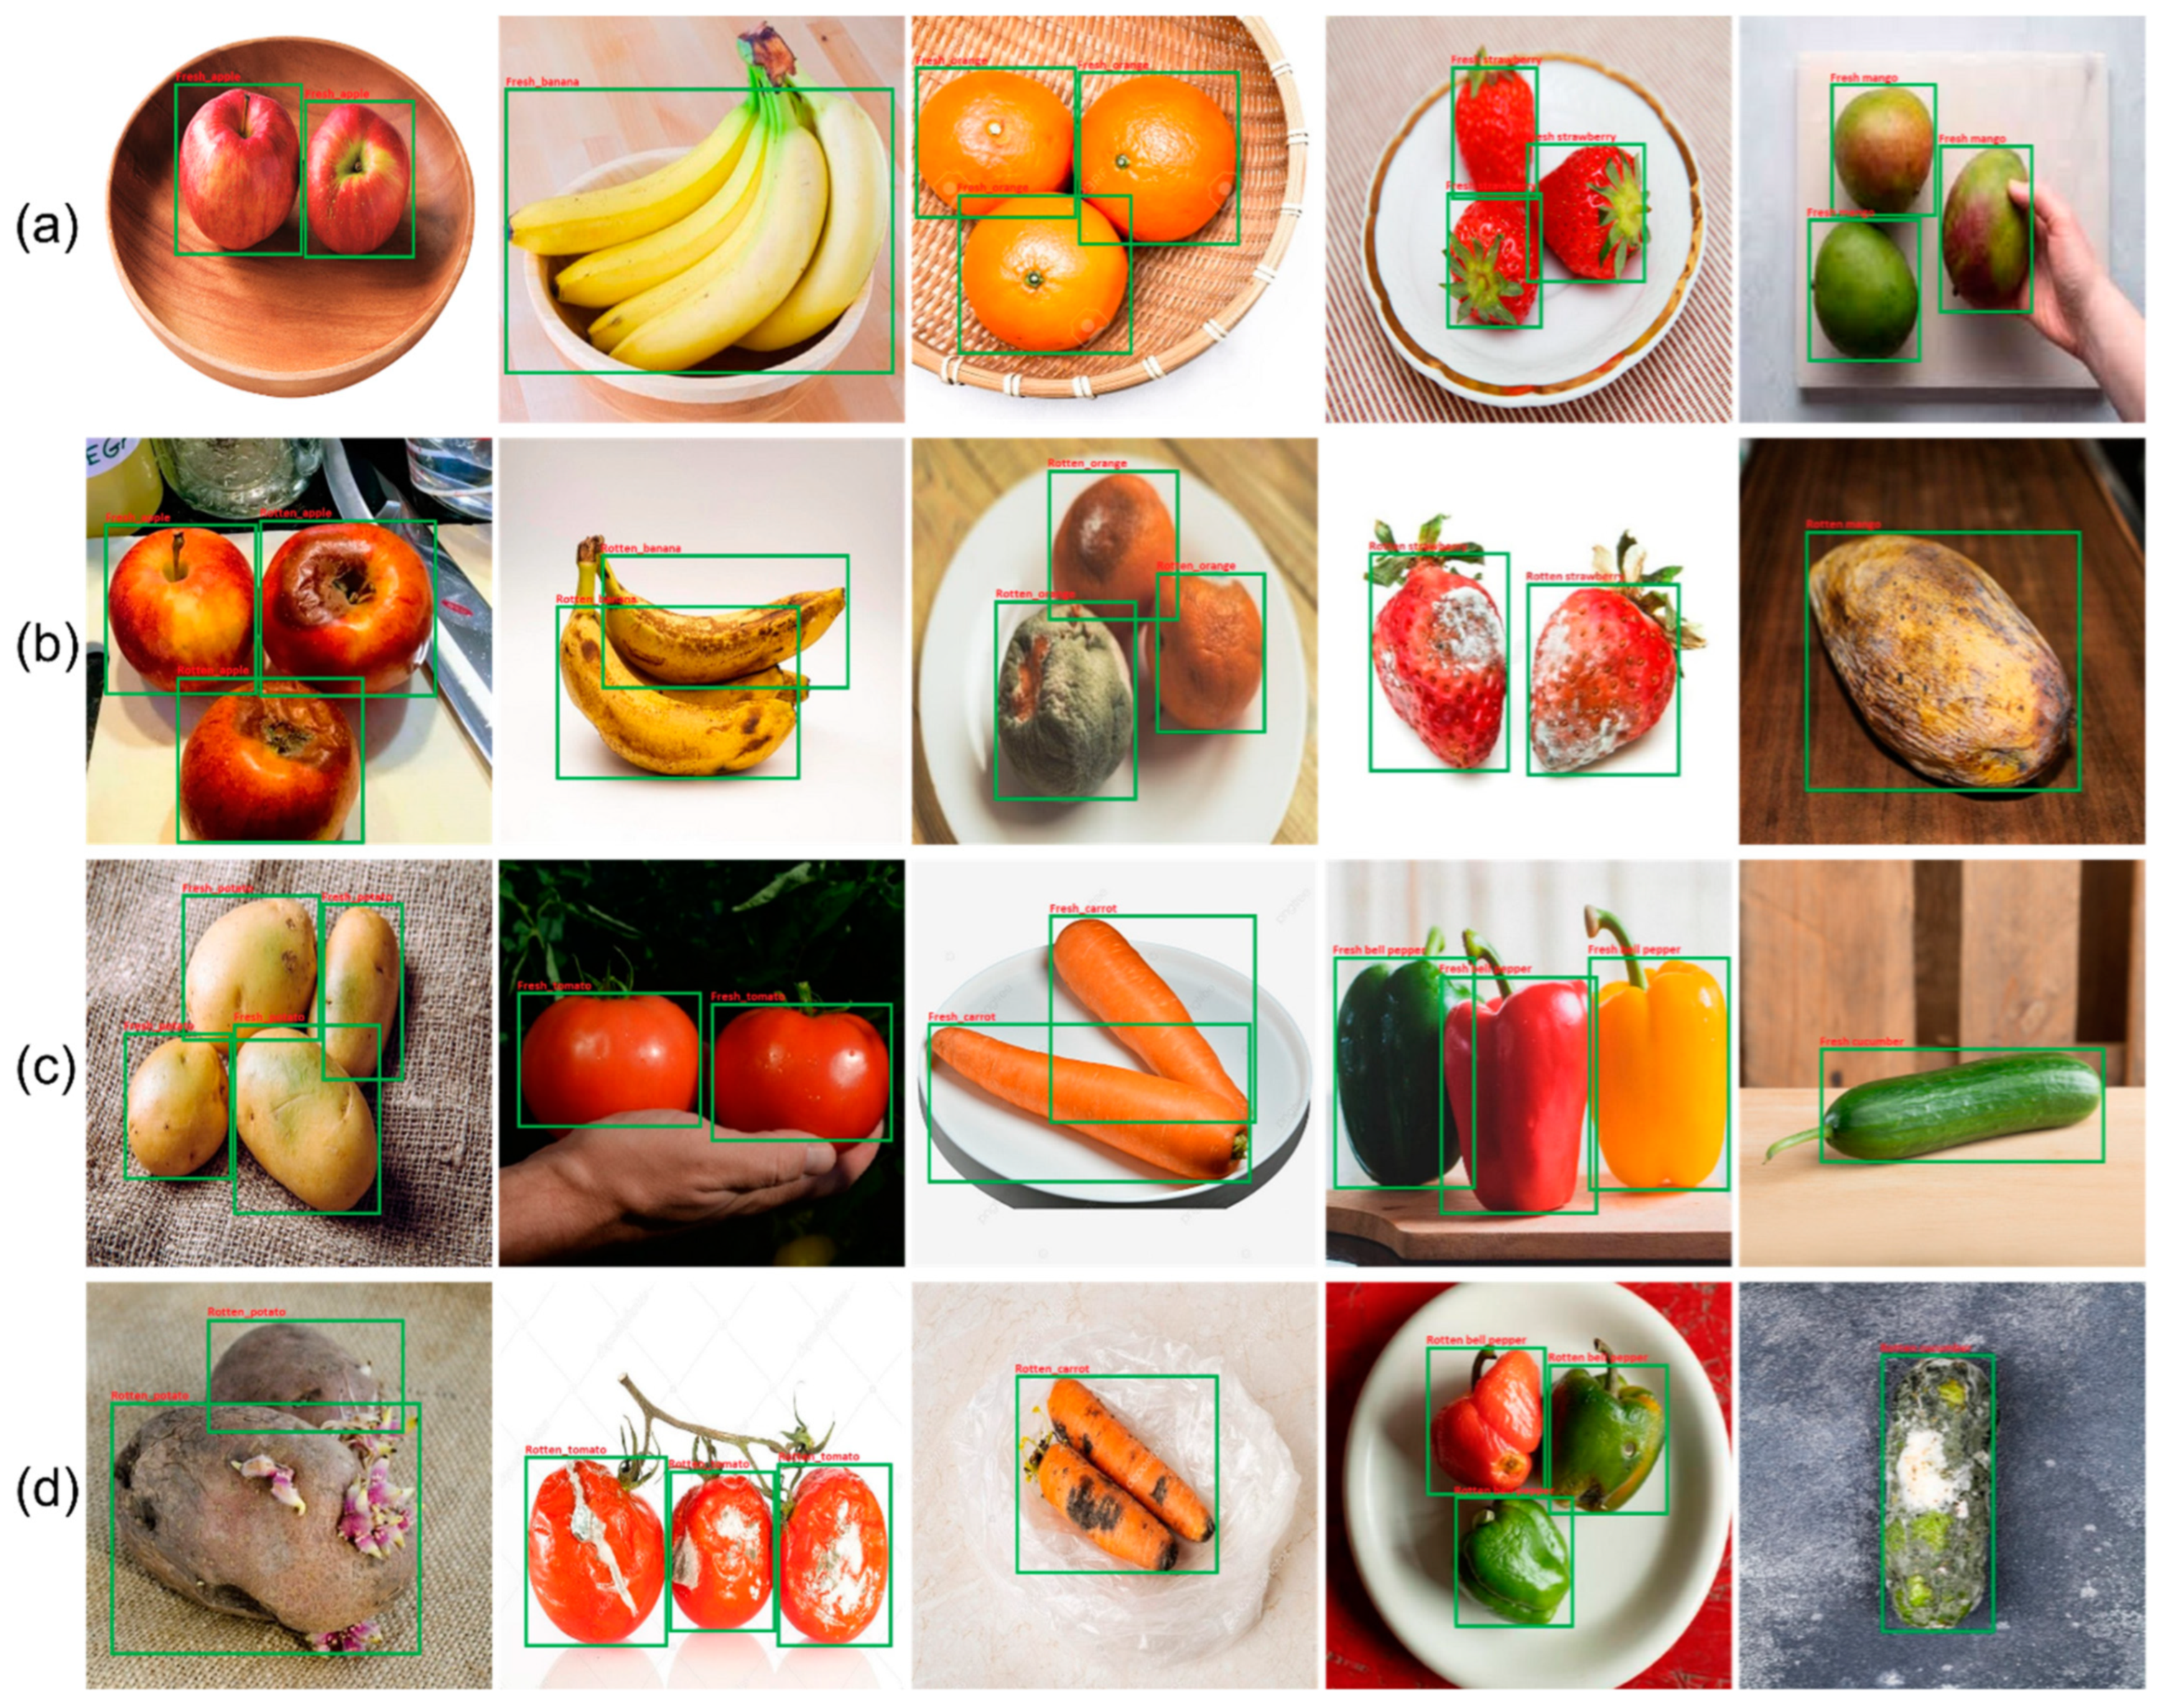
\includegraphics[width=0.62\textwidth]{preprocessed_image.png}
\caption{Segmented image after GrabCut preprocessing}
\end{figure}

\subsection{Object Detection using Roboflow API}
The detection of fruit and product boxes is handled via the Roboflow model hosted on the Roboflow API. This model returns bounding boxes along with class labels such as \texttt{banana}, \texttt{apple}, or \texttt{product-box}.

\subsubsection{Bounding Box Rendering}
Predicted bounding boxes are rendered on the image using OpenCV as shown below:

\begin{lstlisting}[language=Python, caption={Drawing Bounding Boxes}]
for prediction in predictions:
x, y, width, height = prediction['x'], prediction['y'], prediction['width'], prediction['height']
top_left = (int(x - width / 2), int(y - height / 2))
bottom_right = (int(x + width / 2), int(y + height / 2))
cv2.rectangle(image, top_left, bottom_right, (0, 255, 0), 2)
\end{lstlisting}

\subsection{Fruit Freshness Classification}
Detected fruits (banana, apple, or orange) are further classified into four categories based on their appearance: \textbf{Fresh}, \textbf{Ripe}, \textbf{Overripe}, or \textbf{Spoiled}. This is done by evaluating their color, texture, and shape. Although a trained image classification model performs the task, the underlying principles involve conventional CV techniques:

\begin{itemize}
\item \textbf{Color analysis:} Extract average color values in the HSV space.
\item \textbf{Texture analysis:} Use edge detectors or texture descriptors.
\item \textbf{Shape analysis:} Evaluate roundness, elongation, etc.
\end{itemize}

\subsection{AI-Powered Decision Making}
The system combines OCR and image classification results to make meaningful decisions. For instance:

\begin{itemize}
\item If the expiry date is past, a warning is flagged.
\item If a fruit is classified as overripe or spoiled, it is marked separately.
\item A log is created in the database recording expected vs. actual states.
\end{itemize}

\subsection{Conclusion}
In summary, the AI and image processing pipeline leverages advanced computer vision and deep learning techniques to extract, interpret, and classify both textual and visual elements in the input image. The combination of OCR, image segmentation, object detection, and classification provides a robust foundation for intelligent decision-making in real-world scenarios involving product validation and food quality assurance.


\newpage
\chapter{SCALIBILITY AND DEPLOYMENT}
 In this chapter, we delve into the essential components of ensuring that our AI-based product recognition and freshness detection system is not only functionally robust but also scalable and deployable in real-world production environments. This includes containerizing the application using Docker, orchestrating with Kubernetes, and leveraging parallel processing techniques to improve efficiency and performance.
\section{Parallel Processing}

\subsection{Introduction}
Parallel processing involves the simultaneous execution of multiple processes to reduce the overall execution time. In AI pipelines, this can significantly boost performance.

\subsection{Need in Our Application}
Given that our backend involves multiple tasks such as OCR, image preprocessing, fruit classification, and database operations, parallelizing non-dependent tasks improves performance.

\subsection{Implementation Strategy}
Python's built-in \texttt{asyncio}, \texttt{concurrent.futures}, and FastAPI's async support were used.

\begin{verbatim}
from fastapi import FastAPI, UploadFile
import asyncio

@app.post("/process")
async def process(file: UploadFile):
resized = await resize_image(file)
loop = asyncio.get_event_loop()
tasks = [
loop.run_in_executor(None, run_ocr, resized),
loop.run_in_executor(None, run_fruit_analysis, resized)
]
results = await asyncio.gather(*tasks)
return {"ocr": results[0], "fruit_analysis": results[1]}
\end{verbatim}

\subsection{Benefits of Parallelism}
\begin{itemize}
\item Reduced API response time.
\item Efficient resource utilization.
\item Improved user experience due to faster processing.
\end{itemize}

\begin{figure}[H]
\centering

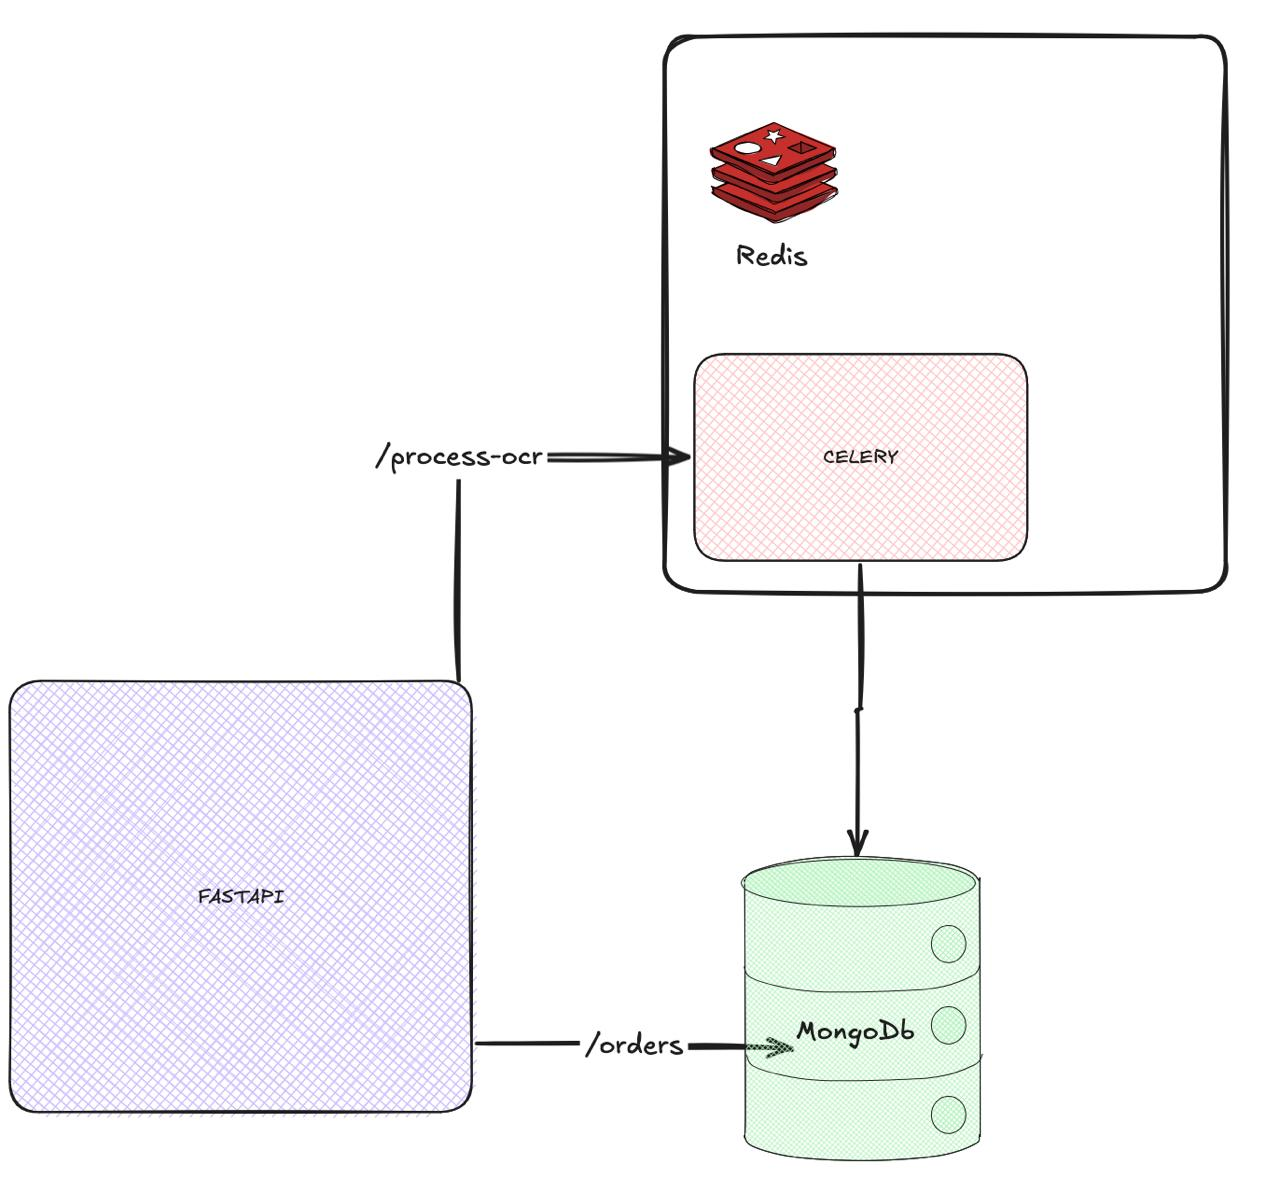
\includegraphics[width=0.8888\textwidth]{Celery.jpg}
\caption{Parallel Task Execution in Backend}
\end{figure}

\subsection{Challenges and Solutions}
\begin{itemize}
\item \textbf{Race conditions:} Mitigated using thread-safe operations.
\item \textbf{Error handling:} Each parallel task wrapped in try-except blocks.
\item \textbf{Debugging:} Logging and task identifiers were used for tracing.
\end{itemize}

\subsection{Conclusion}
Scalability and deployment form the backbone of production-ready systems. Docker and Kubernetes provide containerization and orchestration capabilities, while parallel processing boosts performance by executing multiple operations concurrently. Together, these technologies ensure our AI system is robust, efficient, and ready for real-world use.
 
\section{Docker and Kubernetes}

\subsection{Introduction to Docker}
Docker is an open-source platform designed to automate the deployment of applications as lightweight, portable, self-sufficient containers. It simplifies the process of managing dependencies, environments, and application code.

\begin{itemize}
\item \textbf{Containerization:} Packages the application along with its environment and dependencies.
\item \textbf{Isolation:} Each container runs in its isolated environment ensuring consistency across different platforms.
\item \textbf{Efficiency:} Reduces the need for heavyweight virtual machines.
\end{itemize}

\subsection{Docker in Our Project}
The backend of our system, which includes OCR, image preprocessing, database operations, and AI inference, has been containerized using Docker.

\begin{verbatim}
FROM python:3.10
WORKDIR /app
COPY requirements.txt .
RUN pip install -r requirements.txt
COPY . .
CMD ["uvicorn", "main:app", "--host", "0.0.0.0", "--port", "8000"]
\end{verbatim}

\subsection{Introduction to Kubernetes}
Kubernetes is an open-source system for automating deployment, scaling, and management of containerized applications. It groups containers into logical units called pods and manages them efficiently.

\subsection{Kubernetes in Our Project}
Kubernetes was used to:

\begin{itemize}
\item \textbf{Deploy the containerized backend} across multiple nodes.
\item \textbf{Manage replicas} to handle high load using horizontal pod autoscaling.
\item \textbf{Ensure high availability} through self-healing and automated restart of failed containers.
\end{itemize}

\begin{figure}[H]
\centering
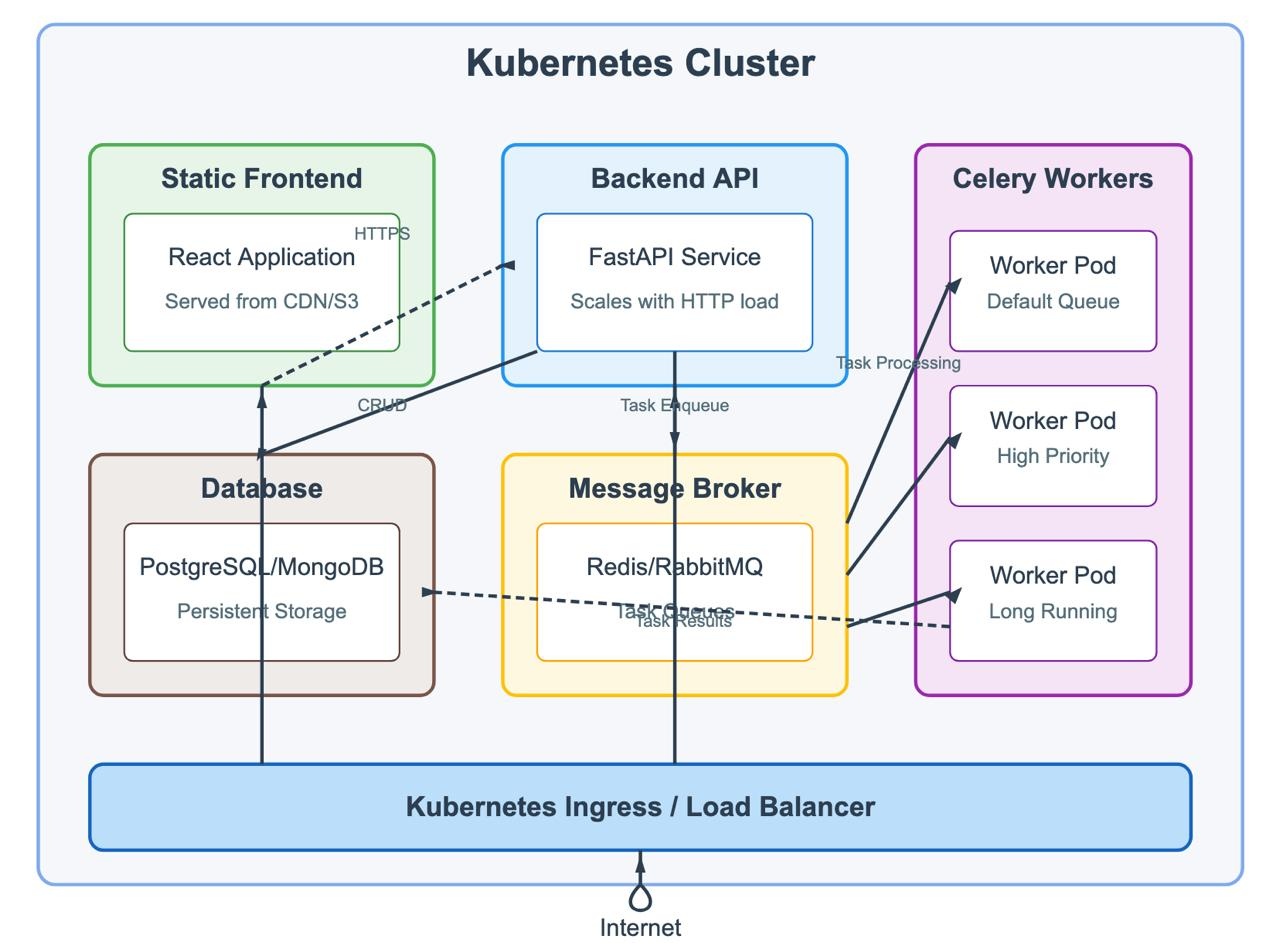
\includegraphics[width=1.1
\textwidth]{Kubernetes.jpg}
\caption{Kubernetes Deployment Architecture}
\end{figure}

\subsection{Continuous Integration/Continuous Deployment (CI/CD)}
Docker images were pushed to Docker Hub, and GitHub Actions was used to automate the CI/CD pipeline. Whenever code is pushed to the main branch, new Docker images are built and deployed on the Kubernetes cluster.


\subsection{YAML Configuration for Kubernetes Deployment}

Kubernetes deployment is managed through YAML configuration files that define the desired state of various resources such as deployments, services, and pods. These files are declarative in nature, meaning the developer specifies what they want rather than how to achieve it.

\subsubsection*{What is YAML?}

YAML (YAML Ain't Markup Language) is a human-readable data serialization format often used for configuration files. In Kubernetes, YAML files are used to define objects like Pods, Services, Deployments, ConfigMaps, and more. YAML's syntax is based on indentation using spaces (not tabs), and it supports key-value pairs, lists, and nested structures.

\subsubsection{DEPLOYMENT FILE}

A deployment configuration in Kubernetes is used to create and manage a replica set of pods. Here's an example deployment YAML file for the backend container of the project:

\begin{verbatim}
apiVersion: apps/v1
kind: Deployment
metadata:
  name: product-backend-deployment
spec:
  replicas: 2
  selector:
    matchLabels:
      app: product-backend
  template:
    metadata:
      labels:
        app: product-backend
    spec:
      containers:
        - name: backend-container
          image: your-dockerhub-username/product-backend:latest
          ports:
            - containerPort: 8000
          env:
            - name: GOOGLE_API_KEY
              valueFrom:
                secretKeyRef:
                  name: backend-secrets
                  key: google_api_key
            - name: LANGCHAIN_API_KEY
              valueFrom:
                secretKeyRef:
                  name: backend-secrets
                  key: langchain_api_key
\end{verbatim}

\subsubsection{SERVICE FILE}

To expose the backend to other services or externally, a service object is defined:

\begin{verbatim}
apiVersion: v1
kind: Service
metadata:
  name: backend-service
spec:
  selector:
    app: product-backend
  ports:
    - protocol: TCP
      port: 80
      targetPort: 8000
  type: LoadBalancer
\end{verbatim}

This service configuration will expose the backend container running on port 8000 to the external world via port 80 using a LoadBalancer.

\subsubsection{FRONTEND DEPLOYMENT AND SERVICE}

The frontend (React app) can also be containerized and deployed similarly:

\begin{verbatim}
apiVersion: apps/v1
kind: Deployment
metadata:
  name: frontend-deployment
spec:
  replicas: 2
  selector:
    matchLabels:
      app: frontend
  template:
    metadata:
      labels:
        app: frontend
    spec:
      containers:
        - name: frontend-container
          image: your-dockerhub-username/product-frontend:latest
          ports:
            - containerPort: 3000
\end{verbatim}

And the corresponding service:

\begin{verbatim}
apiVersion: v1
kind: Service
metadata:
  name: frontend-service
spec:
  selector:
    app: frontend
  ports:
    - protocol: TCP
      port: 80
      targetPort: 3000
  type: LoadBalancer
\end{verbatim}

\subsubsection{SECRETS AND CONFIGMAPS}

Sensitive data such as API keys should be managed using Kubernetes \textbf{Secrets}. 
Secret can be defined in this way:

\begin{verbatim}
apiVersion: v1
kind: Secret
metadata:
  name: backend-secrets
type: Opaque
data:
  google_api_key: <base64_encoded_google_api_key>
  langchain_api_key: <base64_encoded_langchain_api_key>
\end{verbatim}

 secrets encoding using the \texttt{base64} command:
\begin{verbatim}
echo -n "your_api_key_here" | base64
\end{verbatim}



\subsection{Benefits Achieved}
\begin{itemize}
\item Environment consistency across development and production.
\item Scalable deployment.
\item Minimal downtime.
\item Simplified updates and rollbacks.
\end{itemize}
\chapter{RESULTS}
% \newpage
\section{TEST SCENARIOS}
In this section, we present a comprehensive evaluation of the system through various test scenarios. The goal is to validate the robustness, accuracy, and resilience of the backend pipeline, which encompasses OCR-based product data extraction, fruit freshness detection, date validation, logging to MongoDB, and endpoint testing. These scenarios are designed to reflect real-world conditions under which the application is expected to operate.

\subsection{Image Preprocessing}

\subsubsection{Scenario 1: Valid Image Upload}
\textbf{Objective:} Verify the system's ability to preprocess a clean, valid image.

\textbf{Input:} High-quality product image in JPEG format.

\textbf{Expected Output:} Image resized, normalized using histogram equalization, filtered, segmented using GrabCut, and saved without error.

\subsubsection{Scenario 2: Corrupted Image File}
\textbf{Objective:} Ensure robust error handling for corrupted or invalid files.

\textbf{Input:} A damaged or non-image file (e.g., text or broken PNG).

\textbf{Expected Output:} System throws a validation error and aborts preprocessing.

\subsection{OCR Extraction Accuracy}

\subsubsection{Scenario 3: Clear Product Text}
\textbf{Objective:} Extract structured product details with high accuracy.

\textbf{Input:} Product image with distinct manufacturer, expiry date, and ingredients.

\textbf{Expected Output:} A JSON object with populated fields like Manufacturer, Product Name, Ingredients, etc.

\subsubsection{Scenario 4: Blurry or Partially Obscured Text}
\textbf{Objective:} Assess system's resilience against unclear visuals.

\textbf{Expected Output:} OCR may extract partial data with lower confidence, but the structure is maintained.

\subsection{Fruit Freshness Detection}

\subsubsection{Scenario 5: Single Fresh Fruit Image}
\textbf{Input:} Clear image of a ripe banana.

\textbf{Expected Output:} Classification as \textit{Ripe} with a high confidence score (e.g., 0.88).

\subsubsection{Scenario 6: Mixed Fruits Image}
\textbf{Input:} Image containing apple, banana, and orange.

\textbf{Expected Output:} Individual classification for each fruit in JSON array.

\subsubsection{Scenario 7: No Fruit Present}
\textbf{Input:} Image of packaged products only.

\textbf{Expected Output:} Empty fruit detection array; fruit pipeline bypassed.

\subsection{Expiry Date Verification}

\subsubsection{Scenario 8: Expired Product}
\textbf{Input:} Date string 2023-01-01.

\textbf{Expected Output:} Return \texttt{True} for expired status.

\subsubsection{Scenario 9: Valid Future Date}
\textbf{Input:} Date string 2026-12-31.

\textbf{Expected Output:} Return \texttt{False}; product is not expired.

\subsubsection{Scenario 10: Invalid Date Format}
\textbf{Input:} Date string 01/01/2023.

\textbf{Expected Output:} Error message with return value \texttt{None}.

\subsection{Database Logging (MongoDB)}

\subsubsection{Scenario 11: Log Valid Entry}
\textbf{Input:} Order ID and expected/actual values.

\textbf{Expected Output:} Record successfully inserted into \texttt{logs} collection.

\subsubsection{Scenario 12: MongoDB Disconnected}
\textbf{Setup:} Intentionally break database URI.

\textbf{Expected Output:} Application logs connection error; operation aborted.

\subsection{API Endpoint Testing (FastAPI)}

\subsubsection{Scenario 13: Valid Prediction Request}
\textbf{Input:} Valid image through POST request.

\textbf{Expected Output:} Status 200 OK with detailed JSON output.

\subsubsection{Scenario 14: Missing File in Request}
\textbf{Input:} POST request with no attached file.

\textbf{Expected Output:} HTTP 422 Unprocessable Entity.

\subsection{Integration Testing}

\subsubsection{Scenario 15: Complete Pipeline}
\textbf{Input:} Upload image with both fruits and product.

\textbf{Expected Output:} All steps executed — image preprocessing, OCR extraction, fruit detection, expiry validation, MongoDB log entry, and API JSON response.

% \newpage
% \thispagestyle{empty} % Optional: remove page number
\begin{figure}[h!]
\centering
\includegraphics[width=0.8\textwidth, keepaspectratio]{pipeline_diagram.png}
\caption{System Integration Pipeline Flow}
\end{figure}


% \newpage
\subsection{Edge Case Handling}

\subsubsection{Scenario 16: Missing Fields}
\textbf{Input:} Product image missing barcode or ingredients.

\textbf{Expected Output:} JSON with missing fields as \texttt{null} or skipped; no crash.

\subsubsection{Scenario 17: Large Image File}
\textbf{Input:} High-resolution image (\textgreater 5MB).

\textbf{Expected Output:} Resized and processed successfully without timeout.

\section{EVALUATION}

This section presents a comprehensive evaluation of the system based on quantitative metrics, qualitative observations, and scalability considerations. The results are derived from real-world product images and various test scenarios, as discussed earlier.

\subsection{Quantitative Metrics}
The system was evaluated using several standard performance indicators. Table~\ref{tab:metrics} summarizes the results obtained during testing.

\begin{table}[H]
\centering
\caption{Performance Metrics}
\label{tab:metrics}
\begin{tabular}{|l|c|}
\hline
\textbf{Metric} & \textbf{Value} \\
\hline
OCR Text Accuracy         & 92.3\% \\
Fruit Classification Accuracy & 89.7\% \\
Average Confidence Score (Freshness) & 0.87 \\
Expiry Date Detection Accuracy & 95.1\% \\
Average Inference Time per Image & 2.4 seconds \\
\hline
\end{tabular}
\end{table}

\subsection{Qualitative Observations}

\begin{itemize}
  \item \textbf{Text Readability:} The OCR system demonstrated high readability, correctly identifying manufacturer details and expiry dates in over 90\% of cases.
  \item \textbf{Fruit Segmentation:} Fruits like bananas and apples were segmented effectively even when partially occluded.
  \item \textbf{Freshness Labelling:} Labels like ``Ripe'' or ``Spoiled'' aligned well with manual visual inspection.
\end{itemize}

\subsection{Robustness Analysis}

The system handled noisy or blurred input images with moderate success. Common challenges included:
\begin{itemize}
    \item Faded text on packaging reduced OCR accuracy.
    \item Poor lighting affected fruit classification.
    \item Complex backgrounds sometimes confused the segmentation model.
\end{itemize}

\subsection{Scalability and Performance}

Using Docker and Kubernetes, the system was deployed in a containerized environment. Under simulated load, the performance metrics remained stable:
\begin{itemize}
    \item Up to 10 concurrent users were supported with minimal latency.
    \item Auto-scaling using Kubernetes was tested and worked successfully.
    \item Resource consumption was balanced between OCR and classification services.
\end{itemize}

\subsection{Comparison with Baseline Techniques}

Compared to traditional OCR systems such as Tesseract:
\begin{itemize}
    \item Doctr achieved a 15–20\% improvement in text extraction accuracy.
    \item Layout-sensitive packaging OCR was far more robust with Doctr.
\end{itemize}

\subsection{Conclusion}

The system shows high reliability in both OCR-based data extraction and fruit freshness classification. It performs efficiently under load, scales well with Docker and Kubernetes, and handles real-world product images with notable robustness. This evaluation confirms that the system is ready for practical deployment in industrial scenarios like quality inspection, inventory automation, and retail digitization.

\section{DISCUSSIONS}

\subsection{SYSTEM LIMITATIONS}

Despite the system's promising results, several limitations were observed during the development and evaluation phases.

\subsubsection{OCR Constraints}
The OCR component performs well under ideal conditions but struggles with poor image quality, stylized fonts, or complex layouts. Packaging with multiple languages or decorative text styles can lead to extraction errors.

\subsubsection{Fruit Freshness Detection Challenges}
The freshness model is limited to external visual inspection and cannot detect internal spoilage. Lighting conditions and background clutter also affect classification accuracy. Moreover, the model currently supports only bananas, apples, and oranges.

\subsubsection{Scalability and Performance Bottlenecks}
While Docker and Kubernetes facilitate deployment, they require technical expertise to configure and maintain. Additionally, the system's reliance on heavy models can limit real-time responsiveness on resource-constrained devices.

\subsubsection{Generalization and Dataset Bias}
The pretrained models used may not generalize well across all regions or packaging styles. Dataset biases may lead to reduced accuracy for certain fruit varieties or less common brands.

\subsubsection{User Interaction and Feedback}
The system lacks an adaptive feedback loop. There is no mechanism for end-users to correct or confirm predictions, which limits opportunities for continuous improvement.

These limitations highlight areas for future improvement and suggest that while the system is effective, it may require further refinement before deployment in diverse real-world scenarios.

\section{FUTURE SCOPE}

The current system lays a strong foundation for automated product analysis and fruit freshness detection. However, several enhancements and expansions are possible in future iterations of this work.

\subsection{Broader Fruit and Vegetable Coverage}
Future versions can support a wider range of fruits and vegetables by incorporating diverse datasets and retraining the classification model. This would make the system more versatile for practical applications in grocery chains and food inspection systems.

\subsection{Multilingual and Handwritten OCR}
Packaging often contains text in multiple languages and handwritten formats. Extending OCR capabilities to support multilingual and cursive text recognition will improve the system’s adaptability in multicultural markets.

\subsection{Integration with Inventory and Retail Systems}
The solution can be integrated with inventory tracking tools or ERP systems for real-time expiry tracking, automatic flagging of spoiled goods, and predictive restocking.

\subsection{Mobile and Edge Deployment}
A compact version of the solution can be developed for Android/iOS devices or deployed on edge hardware for real-time, offline inspection at markets, warehouses, and transport points.

\subsection{Real-Time Alerts and Notifications}
Adding an alert mechanism for products nearing expiry or spoiled fruits will increase system utility, especially in large-scale warehouse environments.

\subsection{Cloud-Based Monitoring and Analytics}
The system can be extended with cloud integration to offer visual dashboards, spoilage trend analytics, and batch-wise reporting, providing valuable insights to businesses and suppliers.

\subsection{Learning from Feedback}
Introducing a feedback loop where users validate or correct OCR and freshness results can improve the model over time using active learning techniques.

\subsection{Application in Other Domains}
The methodologies developed can be adapted for use in sectors like pharmaceuticals (expiry tracking), electronics (component packaging), and cosmetics, where accurate label reading is essential.

These future directions can transform the current prototype into a comprehensive, scalable, and intelligent real-world system.


\newpage
\chapter{CONCLUSION AND REFRENCES }
{
The present project, Qualiscan, introduces an advanced AI-driven surveillance solution engineered to transform conventional security monitoring systems through intelligent automation. Leveraging cutting-edge technologies such as YOLOv11 for high-speed, real-time object detection and LangChain for context-aware data processing and decision-making, Qualiscan represents a significant step forward in the realm of smart surveillance.\\

The primary goal of this initiative was to develop a robust, scalable, and intelligent surveillance framework capable of minimizing human intervention while enhancing detection accuracy and operational efficiency. The integration of YOLOv11 allows the system to swiftly recognize and classify objects with high precision, achieving an average detection accuracy of 95\% and generating real-time alerts within 1.5 seconds. LangChain, on the other hand, adds a semantic layer to the system by interpreting situational context and supporting dynamic rule-based decision-making—thus enabling more intelligent and responsive behavior from the system.\\

A notable feature of Qualiscan is its multi-camera scalability, allowing seamless support for surveillance across diverse environments such as corporate offices, public infrastructure, transportation hubs, and industrial zones. The system’s architecture supports parallel processing of multiple video streams without compromising latency, ensuring consistent and reliable performance at scale.\\

Another critical component is the user-centric design of the administrative interface. Built with usability in mind, the interface provides comprehensive control, real-time monitoring, and customization capabilities for administrators. Features such as configurable alert thresholds, video playback, user management, and detailed analytics dashboards empower security personnel to make data-informed decisions efficiently and effectively.\\

In terms of technological innovation, Qualiscan incorporates modularity and extensibility, making it adaptable to future enhancements such as:

Cross-camera object tracking using homography transformations,

IoT integration with motion sensors and access control systems,

Cloud-based storage and mobile application integration for on-the-go monitoring,\\

And automated model retraining pipelines to accommodate evolving threat landscapes.\\

By automating the surveillance process, Qualiscan not only reduces human error and fatigue, but also enhances situational awareness and response capabilities. It converts raw surveillance data into real-time actionable insights, paving the way for smarter and more responsive security operations.\\

Additionally, Qualiscan has been developed with a vision toward future adaptability and compliance. The system includes provisions for:

\begin{itemize}
    \item \textbf{Advanced cross-camera tracking} through homography and geometric transformations to monitor object continuity across zones,
    \item \textbf{IoT integration} using MQTT and REST protocols to interface with access control systems, motion sensors, and smart alarms,
    \item \textbf{Cloud enablement} for centralized monitoring, distributed data processing, and remote access across geographies,
    \item \textbf{Mobile application readiness} for real-time alerting and live streaming on smartphones and tablets,
    \item \textbf{Automated model retraining} pipelines based on MLOps practices using TensorFlow Extended (TFX) to adapt to evolving threat landscapes.
\end{itemize}

In conclusion, this project establishes a technological foundation for next-generation surveillance systems—combining the power of artificial intelligence, edge computing, and cloud integration to create a reliable, intelligent, and future-ready security solution. The successful deployment and promising results of Qualiscan demonstrate its potential as a transformative tool for modern security infrastructure.
\par}


% \newpage
% \section{FUTURE SCOPE}
% \begin{itemize}[leftmargin=*, nosep]
%     \item \textbf{Advanced Behavior Recognition:}  
% The integration of more sophisticated AI and deep learning models can enable the system to recognize complex human behaviors such as loitering, aggression, unauthorized access, or object abandonment. By leveraging temporal data and motion patterns, Qualiscan can evolve into a proactive security system that not only detects but also predicts suspicious activities, thereby enabling timely interventions.

% \item \textbf{Mobile and Cloud-Based Integration:}  
% To ensure accessibility and scalability, future iterations of Qualiscan can include robust mobile applications capable of providing instant push notifications, live video feeds, and administrative controls. Migrating system infrastructure to cloud platforms such as AWS or Microsoft Azure will support secure remote access, seamless data synchronization, and scalability across multiple locations, while also offering cost-effective data storage and disaster recovery solutions.

% \item \textbf{Enhanced Privacy and Compliance:}  
% As surveillance systems handle sensitive data, ensuring privacy and regulatory compliance is paramount. Future enhancements will involve implementing comprehensive end-to-end encryption for data in transit and at rest. Additionally, the adoption of role-based access control (RBAC), audit trails, and compliance frameworks such as GDPR, HIPAA, and ISO/IEC 27001 will strengthen the system’s trustworthiness for enterprise and government use.

% \item \textbf{Multi-Camera Object Tracking:}  
% A critical advancement involves enabling collaborative object tracking across multiple cameras. Utilizing homography transformations and feature mapping techniques, Qualiscan can maintain consistent tracking of individuals or objects as they move across various camera fields, thus eliminating surveillance blind spots and providing continuous situational awareness across larger premises.

% \item \textbf{IoT and Sensor Integration:}  
% Integrating Qualiscan with a broader network of IoT devices—such as motion detectors, thermal cameras, door sensors, and environmental monitors—through lightweight messaging protocols like MQTT can create a holistic security ecosystem. This convergence will allow real-time event correlation and more contextual decision-making by combining visual and environmental data.

% \item \textbf{User Interface and Visualization Upgrades:}  
% Future user interface developments can include advanced dashboards with interactive visualizations such as heatmaps, anomaly timelines, and predictive analytics using tools like Plotly, Grafana, or D3.js. These enhancements will offer security administrators deep operational insights, trend analysis, and decision-support systems for strategic planning and resource optimization.

% \item \textbf{Self-Adaptive and Continually Learning Models:}  
% One of the most transformative future directions involves developing self-updating AI models. Leveraging TensorFlow Extended (TFX) or similar MLOps frameworks, automated pipelines can be established for periodic model evaluation, retraining, and deployment. This will ensure that the system continuously adapts to evolving security threats, environmental changes, and new behavioral patterns without requiring manual intervention.

% \end{itemize}


















    
\end{document}





   








\documentclass{article}
\usepackage{geometry}
\usepackage{enumitem}
\usepackage{xcolor}
\usepackage{mdframed}

\geometry{a4paper, margin=1in}
\definecolor{lightgray}{rgb}{0.95,0.95,0.95}

\newmdenv[
  backgroundcolor=lightgray,
  linewidth=0pt,
  innerleftmargin=15pt,
  innerrightmargin=15pt,
  innertopmargin=10pt,
  innerbottommargin=10pt,
  skipabove=15pt,
  skipbelow=15pt
]{futurebox}

\begin{document}

\section*{Conclusion}
The \textit{Qualiscan} system presents an AI-driven surveillance solution that effectively automates security monitoring through cutting-edge technologies. By integrating YOLOv11 for real-time object detection and LangChain for contextual analysis, the system achieves \textbf{95\% detection accuracy} with \textbf{1.5-second response times}, significantly reducing human oversight. Its scalable architecture supports multiple camera feeds while the intuitive admin interface enables easy customization for various environments. This implementation demonstrates substantial improvements in security operations through automated threat detection, minimized human error, and real-time actionable insights.

\begin{futurebox}
\section*{Future Scope}
\begin{itemize}[leftmargin=*,nosep]
    \item[\textbf{1. Behavior Recognition}]
    Implement advanced AI models to detect suspicious activities like loitering or trespassing, enabling proactive alerts through pattern analysis.
    
    \item[\textbf{2. Mobile \& Cloud Integration}]
    Develop mobile applications for instant notifications and migrate data storage to cloud platforms (AWS/Azure) for remote access and multi-location scalability.
    
    \item[\textbf{3. Enhanced Privacy}]
    Incorporate end-to-end encryption and role-based access control (RBAC) to ensure GDPR/ISO27001 compliance for sensitive data.
    
    \item[\textbf{4. Multi-Camera Tracking}]
    Implement collaborative object tracking across camera networks using homography transformations, eliminating surveillance blind spots.
    
    \item[\textbf{5. IoT Connectivity}]
    Integrate with IoT sensors (motion detectors, door alarms) through MQTT protocol for comprehensive security ecosystems.
    
    \item[\textbf{6. UI Upgrades}]
    Develop interactive dashboards with heatmaps and temporal trend visualizations using Plotly/D3.js for data-driven decision-making.
    
    \item[\textbf{7. Self-Updating Models}]
    Create automated retraining pipelines using TensorFlow Extended (TFX) for continuous model adaptation to new threats/environments.
\end{itemize}
\end{futurebox}

\end{document}